%%%%%%%%%%%%%%%%%%%%%%%%%%%%%%%%%%%%%%%%%%%%%%%%%%%%%%%%%%%%%%%
%% OXFORD THESIS TEMPLATE

% Use this template to produce a standard thesis that meets the Oxford University requirements for DPhil submission
%
% Originally by Keith A. Gillow (gillow@maths.ox.ac.uk), 1997
% Modified by Sam Evans (sam@samuelevansresearch.org), 2007
% Modified by John McManigle (john@oxfordechoes.com), 2015
% Modified by Anna James-Bott, 2020-2021
%
% This version Copyright (c) 2015-2017 John McManigle
%
% Broad permissions are granted to use, modify, and distribute this software
% as specified in the MIT License included in this distribution's LICENSE file.
%

% I've (John) tried to comment this file extensively, so read through it to see how to use the various options.  Remember
% that in LaTeX, any line starting with a % is NOT executed.  Several places below, you have a choice of which line to use
% out of multiple options (eg draft vs final, for PDF vs for binding, etc.)  When you pick one, add a % to the beginning of
% the lines you don't want.


%%%%% CHOOSE PAGE LAYOUT
% The most common choices should be below.  You can also do other things, like replacing "a4paper" with "letterpaper", etc.

% This one will format for two-sided binding (ie left and right pages have mirror margins; blank pages inserted where needed):
%\documentclass[a4paper,twoside]{ociamthesis}
% This one will format for one-sided binding (ie left margin > right margin; no extra blank pages):
%\documentclass[a4paper]{ociamthesis}
% This one will format for PDF output (ie equal margins, no extra blank pages):
\documentclass[a4paper,nobind]{ociamthesis}



%%%%% SELECT YOUR DRAFT OPTIONS
% Three options going on here; use in any combination.  But remember to turn the first two off before
% generating a PDF to send to the printer!

% This adds a "DRAFT" footer to every normal page.  (The first page of each chapter is not a "normal" page.)
\fancyfoot[C]{\emph{DRAFT Printed on \today}}

% This highlights (in blue) corrections marked with (for words) \mccorrect{blah} or (for whole
% paragraphs) \begin{mccorrection} . . . \end{mccorrection}.  This can be useful for sending a PDF of
% your corrected thesis to your examiners for review.  Turn it off, and the blue disappears.
\correctionstrue


%%%%% BIBLIOGRAPHY SETUP
% Note that your bibliography will require some tweaking depending on your department, preferred format, etc.
% The options included below are just very basic "sciencey" and "humanitiesey" options to get started.
% If you've not used LaTeX before, I recommend reading a little about biblatex/biber and getting started with it.
% If you're already a LaTeX pro and are used to natbib or something, modify as necessary.
% Either way, you'll have to choose and configure an appropriate bibliography format...

% The science-type option: numerical in-text citation with references in order of appearance.
\usepackage[style=numeric-comp, sorting=none, backend=biber, doi=false, isbn=false]{biblatex}
\newcommand*{\bibtitle}{References}

% The humanities-type option: author-year in-text citation with an alphabetical works cited.
%\usepackage[style=authoryear, sorting=nyt, backend=biber, maxcitenames=2, useprefix, doi=false, isbn=false]{biblatex}
%\newcommand*{\bibtitle}{Works Cited}

% This makes the bibliography left-aligned (not 'justified') and slightly smaller font.
\renewcommand*{\bibfont}{\raggedright\small}

% Change this to the name of your .bib file (usually exported from a citation manager like Zotero or EndNote).
% \addbibresource{references.bib} % Overall bib file
\addbibresource{bib_introduction.bib}
\addbibresource{bib_methods.bib}



%\printbibliography[heading=bibintoc,title={\bibtitle}]}

% Uncomment this if you want equation numbers per section (2.3.12), instead of per chapter (2.18):
%\numberwithin{equation}{subsection}



%%%%% THESIS / TITLE PAGE INFORMATION
% Everybody needs to complete the following:
\title{Using a multi-omics approach to investigate the reversal of proteasome inhibitor drug resistance in multiple myeloma with epigenetic inhibitors}
\author{Anna James-Bott}
\college{St Hilda's College}


% Uncomment the following line if your degree also includes exams (eg most masters):
%\renewcommand{\submittedtext}{Submitted in partial completion of the}
% Your full degree name.  (But remember that DPhils aren't "in" anything.  They're just DPhils.)
\degree{Doctor of Philosophy}
% Term and year of submission, or date if your board requires (eg most masters)
\degreedate{Trinity 2021}


%%%%% YOUR OWN PERSONAL MACROS
% This is a good place to dump your own LaTeX macros as they come up.

% To make text superscripts shortcuts
	\renewcommand{\th}{\textsuperscript{th}} % ex: I won 4\th place
	\newcommand{\nd}{\textsuperscript{nd}}
	\renewcommand{\st}{\textsuperscript{st}}
	\newcommand{\rd}{\textsuperscript{rd}}

% Must be placed before `minitoc` is loaded!
\newcommand{\minitocpath}{%
  minitocdump/% Change the name of the directory.
}

%%%%% THE ACTUAL DOCUMENT STARTS HERE
\begin{document}



%%%%% CHOOSE YOUR LINE SPACING HERE
% This is the official option.  Use it for your submission copy and library copy:
\setlength{\textbaselineskip}{22pt plus2pt}
% This is closer spacing (about 1.5-spaced) that you might prefer for your personal copies:
%\setlength{\textbaselineskip}{18pt plus2pt minus1pt}

% You can set the spacing here for the roman-numbered pages (acknowledgements, table of contents, etc.)
\setlength{\frontmatterbaselineskip}{17pt plus1pt minus1pt}

% Leave this line alone; it gets things started for the real document.
\setlength{\baselineskip}{\textbaselineskip}


%%%%% CHOOSE YOUR SECTION NUMBERING DEPTH HERE
% You have two choices.  First, how far down are sections numbered?  (Below that, they're named but
% don't get numbers.)  Second, what level of section appears in the table of contents?  These don't have
% to match: you can have numbered sections that don't show up in the ToC, or unnumbered sections that
% do.  Throughout, 0 = chapter; 1 = section; 2 = subsection; 3 = subsubsection, 4 = paragraph...

% The level that gets a number:
\setcounter{secnumdepth}{2}
% The level that shows up in the ToC:
\setcounter{tocdepth}{2}


%%%%% ABSTRACT SEPARATE
% This is used to create the separate, one-page abstract that you are required to hand into the Exam
% Schools.  You can comment it out to generate a PDF for printing or whatnot.
%\begin{abstractseparate}
%	%Standardised robust wet-lab and computational single-cell workflows will be established to characterise drug-resistant MM cells

Multiple myeloma (MM) is an incurable cancer of plasma cells, with an average five-year survival rate of approximately 50\%.
Over the last two decades application of now standard MM therapeutics, namely proteasome inhibitors (PI) and immunomodulatory imide drugs (IMiD), have almost doubled median survival time of MM patients.
However, most patients relapse and become resistant to drugs they previously have been treated with.
Acquired anti-cancer drug resistance remains one of the biggest barriers in the treatment of myeloma.
Therefore, identifying novel therapeutics effective against MM, which are capable of overcoming drug resistance is of the utmost importance.
Recently the prolyl-tRNA synthetase inhibitor, Halofuginone, has been shown to be effective against cancer, including one study demonstrating effectiveness against MM\@.





% old shit rip
%Recently, epigenetic mechanisms have been implicated in both the onset of MM and in the development of drug resistance.
%This thesis aims to investigate the changes that drive proteasome inhibitor drug resistance and to identify epigenetic compounds capable of reversing the resistance phenotype, and characterise their mechanism of action.
%The model MM cell line, AMO-1 was used in this work.
%Following an epigenetic compound library screen and bulk RNA-seq, a dual TRIM24/BRPF inhibitor (TRIM24i) was selected to be investigated further as it was shown to kill carfilzomib-resistant AMO-1 cells (aCFZ) in the presence of carfilzomib but had little effect on PI-sensitive (WT) AMO-1 cells, demonstrating that it is capable of re-sensitizing carfilzomib-resistant AMO-1 cells to carfilzomib.
%Transcriptomic, epigenomic and proteomic changes were studied using an array of `omic' techniques, including bulk and single-cell RNA-Seq, phosphoproteomics, ubiquitinomics, total proteomics, CyTOF and ChIP-Seq (PROBABLY will at some point).

 % Create an abstract.tex file in the 'text' folder for your abstract.
%\end{abstractseparate}


% JEM: Pages are roman numbered from here, though page numbers are invisible until ToC.  This is in
% keeping with most typesetting conventions.
\begin{romanpages}

% Title page is created here
\maketitle

%%%%% DEDICATION -- If you'd like one, un-comment the following.
%\begin{dedication}
%This thesis is dedicated to\\
%someone\\
%for some special reason\\
%\end{dedication}

%%%%% ACKNOWLEDGEMENTS -- Nothing to do here except comment out if you don't want it.
\begin{acknowledgements}
 	\subsection*{Personal}

This is where you thank your advisor, colleagues, and family and friends.

Lorem ipsum dolor sit amet, consectetur adipiscing elit. Vestibulum feugiat et est at accumsan. Praesent sed elit mattis, congue mi sed, porta ipsum. In non ullamcorper lacus. Quisque volutpat tempus ligula ac ultricies. Nam sed erat feugiat, elementum dolor sed, elementum neque. Aliquam eu iaculis est, a sollicitudin augue. Cras id lorem vel purus posuere tempor. Proin tincidunt, sapien non dictum aliquam, ex odio ornare mauris, ultrices viverra nisi magna in lacus. Fusce aliquet molestie massa, ut fringilla purus rutrum consectetur. Nam non nunc tincidunt, rutrum dui sit amet, ornare nunc. Donec cursus tortor vel odio molestie dignissim. Vivamus id mi erat. Duis porttitor diam tempor rutrum porttitor. Lorem ipsum dolor sit amet, consectetur adipiscing elit. Sed condimentum venenatis consectetur. Lorem ipsum dolor sit amet, consectetur adipiscing elit.

Aenean sit amet lectus nec tellus viverra ultrices vitae commodo nunc. Mauris at maximus arcu. Aliquam varius congue orci et ultrices. In non ipsum vel est scelerisque efficitur in at augue. Nullam rhoncus orci velit. Duis ultricies accumsan feugiat. Etiam consectetur ornare velit et eleifend.

Suspendisse sed enim lacinia, pharetra neque ac, ultricies urna. Phasellus sit amet cursus purus. Quisque non odio libero. Etiam iaculis odio a ex volutpat, eget pulvinar augue mollis. Mauris nibh lorem, mollis quis semper quis, consequat nec metus. Etiam dolor mi, cursus a ipsum aliquam, eleifend venenatis ipsum. Maecenas tempus, nibh eget scelerisque feugiat, leo nibh lobortis diam, id laoreet purus dolor eu mauris. Pellentesque habitant morbi tristique senectus et netus et malesuada fames ac turpis egestas. Nulla eget tortor eu arcu sagittis euismod fermentum id neque. In sit amet justo ligula. Donec rutrum ex a aliquet egestas.

\subsection*{Institutional}

If you want to separate out your thanks for funding and institutional support, I don't think there's any rule against it.  Of course, you could also just remove the subsections and do one big traditional acknowledgement section.

Lorem ipsum dolor sit amet, consectetur adipiscing elit. Ut luctus tempor ex at pretium. Sed varius, mauris at dapibus lobortis, elit purus tempor neque, facilisis sollicitudin felis nunc a urna. Morbi mattis ante non augue blandit pulvinar. Quisque nec euismod mauris. Nulla et tellus eu nibh auctor malesuada quis imperdiet quam. Sed eget tincidunt velit. Cras molestie sem ipsum, at faucibus quam mattis vel. Quisque vel placerat orci, id tempor urna. Vivamus mollis, neque in aliquam consequat, dui sem volutpat lorem, sit amet tempor ipsum felis eget ante. Integer lacinia nulla vitae felis vulputate, at tincidunt ligula maximus. Aenean venenatis dolor ante, euismod ultrices nibh mollis ac. Ut malesuada aliquam urna, ac interdum magna malesuada posuere.
\end{acknowledgements}

%%%%% ABSTRACT -- Nothing to do here except comment out if you don't want it.
\begin{abstract}
	%Standardised robust wet-lab and computational single-cell workflows will be established to characterise drug-resistant MM cells

Multiple myeloma (MM) is an incurable cancer of plasma cells, with an average five-year survival rate of approximately 50\%.
Over the last two decades application of now standard MM therapeutics, namely proteasome inhibitors (PI) and immunomodulatory imide drugs (IMiD), have almost doubled median survival time of MM patients.
However, most patients relapse and become resistant to drugs they previously have been treated with.
Acquired anti-cancer drug resistance remains one of the biggest barriers in the treatment of myeloma.
Therefore, identifying novel therapeutics effective against MM, which are capable of overcoming drug resistance is of the utmost importance.
Recently the prolyl-tRNA synthetase inhibitor, Halofuginone, has been shown to be effective against cancer, including one study demonstrating effectiveness against MM\@.





% old shit rip
%Recently, epigenetic mechanisms have been implicated in both the onset of MM and in the development of drug resistance.
%This thesis aims to investigate the changes that drive proteasome inhibitor drug resistance and to identify epigenetic compounds capable of reversing the resistance phenotype, and characterise their mechanism of action.
%The model MM cell line, AMO-1 was used in this work.
%Following an epigenetic compound library screen and bulk RNA-seq, a dual TRIM24/BRPF inhibitor (TRIM24i) was selected to be investigated further as it was shown to kill carfilzomib-resistant AMO-1 cells (aCFZ) in the presence of carfilzomib but had little effect on PI-sensitive (WT) AMO-1 cells, demonstrating that it is capable of re-sensitizing carfilzomib-resistant AMO-1 cells to carfilzomib.
%Transcriptomic, epigenomic and proteomic changes were studied using an array of `omic' techniques, including bulk and single-cell RNA-Seq, phosphoproteomics, ubiquitinomics, total proteomics, CyTOF and ChIP-Seq (PROBABLY will at some point).


\end{abstract}

%%%%% MINI TABLES
% This lays the groundwork for per-chapter, mini tables of contents.  Comment the following line
% (and remove \minitoc from the chapter files) if you don't want this.  Un-comment either of the
% next two lines if you want a per-chapter list of figures or tables.
%\dominitoc % include a mini table of contents
%\dominilof  % include a mini list of figures
%\dominilot  % include a mini list of tables

% This aligns the bottom of the text of each page.  It generally makes things look better.
\flushbottom

% This is where the whole-document ToC appears:
\tableofcontents

\listoffigures
	\mtcaddchapter
% \mtcaddchapter is needed when adding a non-chapter (but chapter-like) entity to avoid confusing minitoc

% Uncomment to generate a list of tables:
\listoftables
	\mtcaddchapter

%%%%% LIST OF ABBREVIATIONS
% This example includes a list of abbreviations.  Look at text/abbreviations.tex to see how that file is
% formatted.  The template can handle any kind of list though, so this might be a good place for a
% glossary, etc.
% First parameter can be changed eg to "Glossary" or something.
% Second parameter is the max length of bold terms.
\begin{mclistof}{List of Abbreviations}{3.2cm}

\item[MM] Multiple Myeloma

\item[BM] Bone marrow

\item[MGUS] Monoclonal gammopathy of unknown significance

\item[SMM] Smoldering multiple myeloma

\item[PI] Proteasome inhibitor

\item[IMiDs] Immunomodulatory imide drugs

\item[ER] Endoplasmic reticulum

\item[UPS] Ubiquitin proteasome system

\item[UPR] Unfolded protein response

\item[DNA] Deoxyribonucleic acid

\item[RNA] Ribonucleic acid

\item[NGS] Next generation sequencing

\item[WGS] Whole genome sequencing

\item[RNA-Seq] Ribonucleic acid sequencing

\item[scRNA-Seq] Single cell RNA-Seq

\item[dscRNA-Seq] Droplet-based scRNA-Seq

\item[CB] Cellular barcode

\item[UMI] Unique molecular identifier

\item[LC-MS/MS] Liquid chromatography with tandem mass spectrometry

\item[PCA] Principle component analysis

\item[DMSO] Dimethyl sulfoxide

\item[UMAP] Uniform Manifold Approximation and Projection

\item[tSNE] t-distributed Stochastic Neighbor Embedding

\end{mclistof} 


% The Roman pages, like the Roman Empire, must come to its inevitable close.
\end{romanpages}


%%%%% CHAPTERS
% Add or remove any chapters you'd like here, by file name (excluding '.tex'):
\flushbottom
\chapter{\label{ch:1-intro}Introduction} 

%\minitoc

\section{Overview}
...

% 1
\section{The adaptive immune system}
Humans are exposed to millions of potential pathogens every day and therefore require defences to be able to protect themselves against infection.
These defences can be innate or adaptive.
An example of an innate defence is the skin acting as a physical barrier between the outside world and the body.
Another example of an innate defence is non-specific engulfing (phagocytosis) of foreign pathogens by macrophages (a type of white blood cell).
Innate responses are relied upon as the first line of defence, however sometimes a more sophisticated, specialised response is required- called the adaptive immune response. (REF-mol biology of the cell).

Adaptive immune responses are specific to the pathogen that induced the response and are dependent on B cells and T cells, two major classes of lymphocytes (a class of white blood cell).
Two classes of adaptive immune responses exist: antibody responses, co-ordinated by B cells, and cell mediated immune responses, co-ordinated by T cells.
T-cell-mediated immune responses recognise foreign antigens (antibody generators;
substances capable of eliciting an immune response by stimulating B or T cell activation) on the surface of cells and can either kill the pathogen-infected cells or stimulate B cells or phagocytes to help eliminate the pathogen.
In antibody responses, B cells and plasma cells secrete antibodies, also known as immunoglobulins.
Immunoglobulins are large Y-shaped proteins, which recognise and bind to the specific foreign antigen on the pathogen which stimulated their production.
Binding of immunoglobulins to antigens renders the virus or microbial toxin inactive as it blocks their ability to bind to host cells.
Additionally, antibody binding makes it easier for phagocytic cells to ingest the pathogen.
%%%%%%


%2
\subsection{Plasma cells}
%3
\subsubsection{Plasma cell development}
Stem cells are precursor cells which can give rise to at least one type of differentiated (mature) cell, with the capability of indefinite self-renewal.
Hematopoietic stem cells (HSC) are stem cells that give rise to all the cells of the hematopoietic system.
Two predominant cell populations are produced by HSCs: the common myeloid progenitor (CMP) and the common lymphocyte progenitor (CLP).
CMP differentiation produces erythrocytes (red blood cells), mast cells, monocytes, macrophages, neutrophils, eosinophils, basophils and myeloid dendritic cells.
CLP differentiation results in B cells, T cells, natural killer (NK) cells and lymphoid dendritic cells.

%% Immune cell figure
\begin{figure}
\centering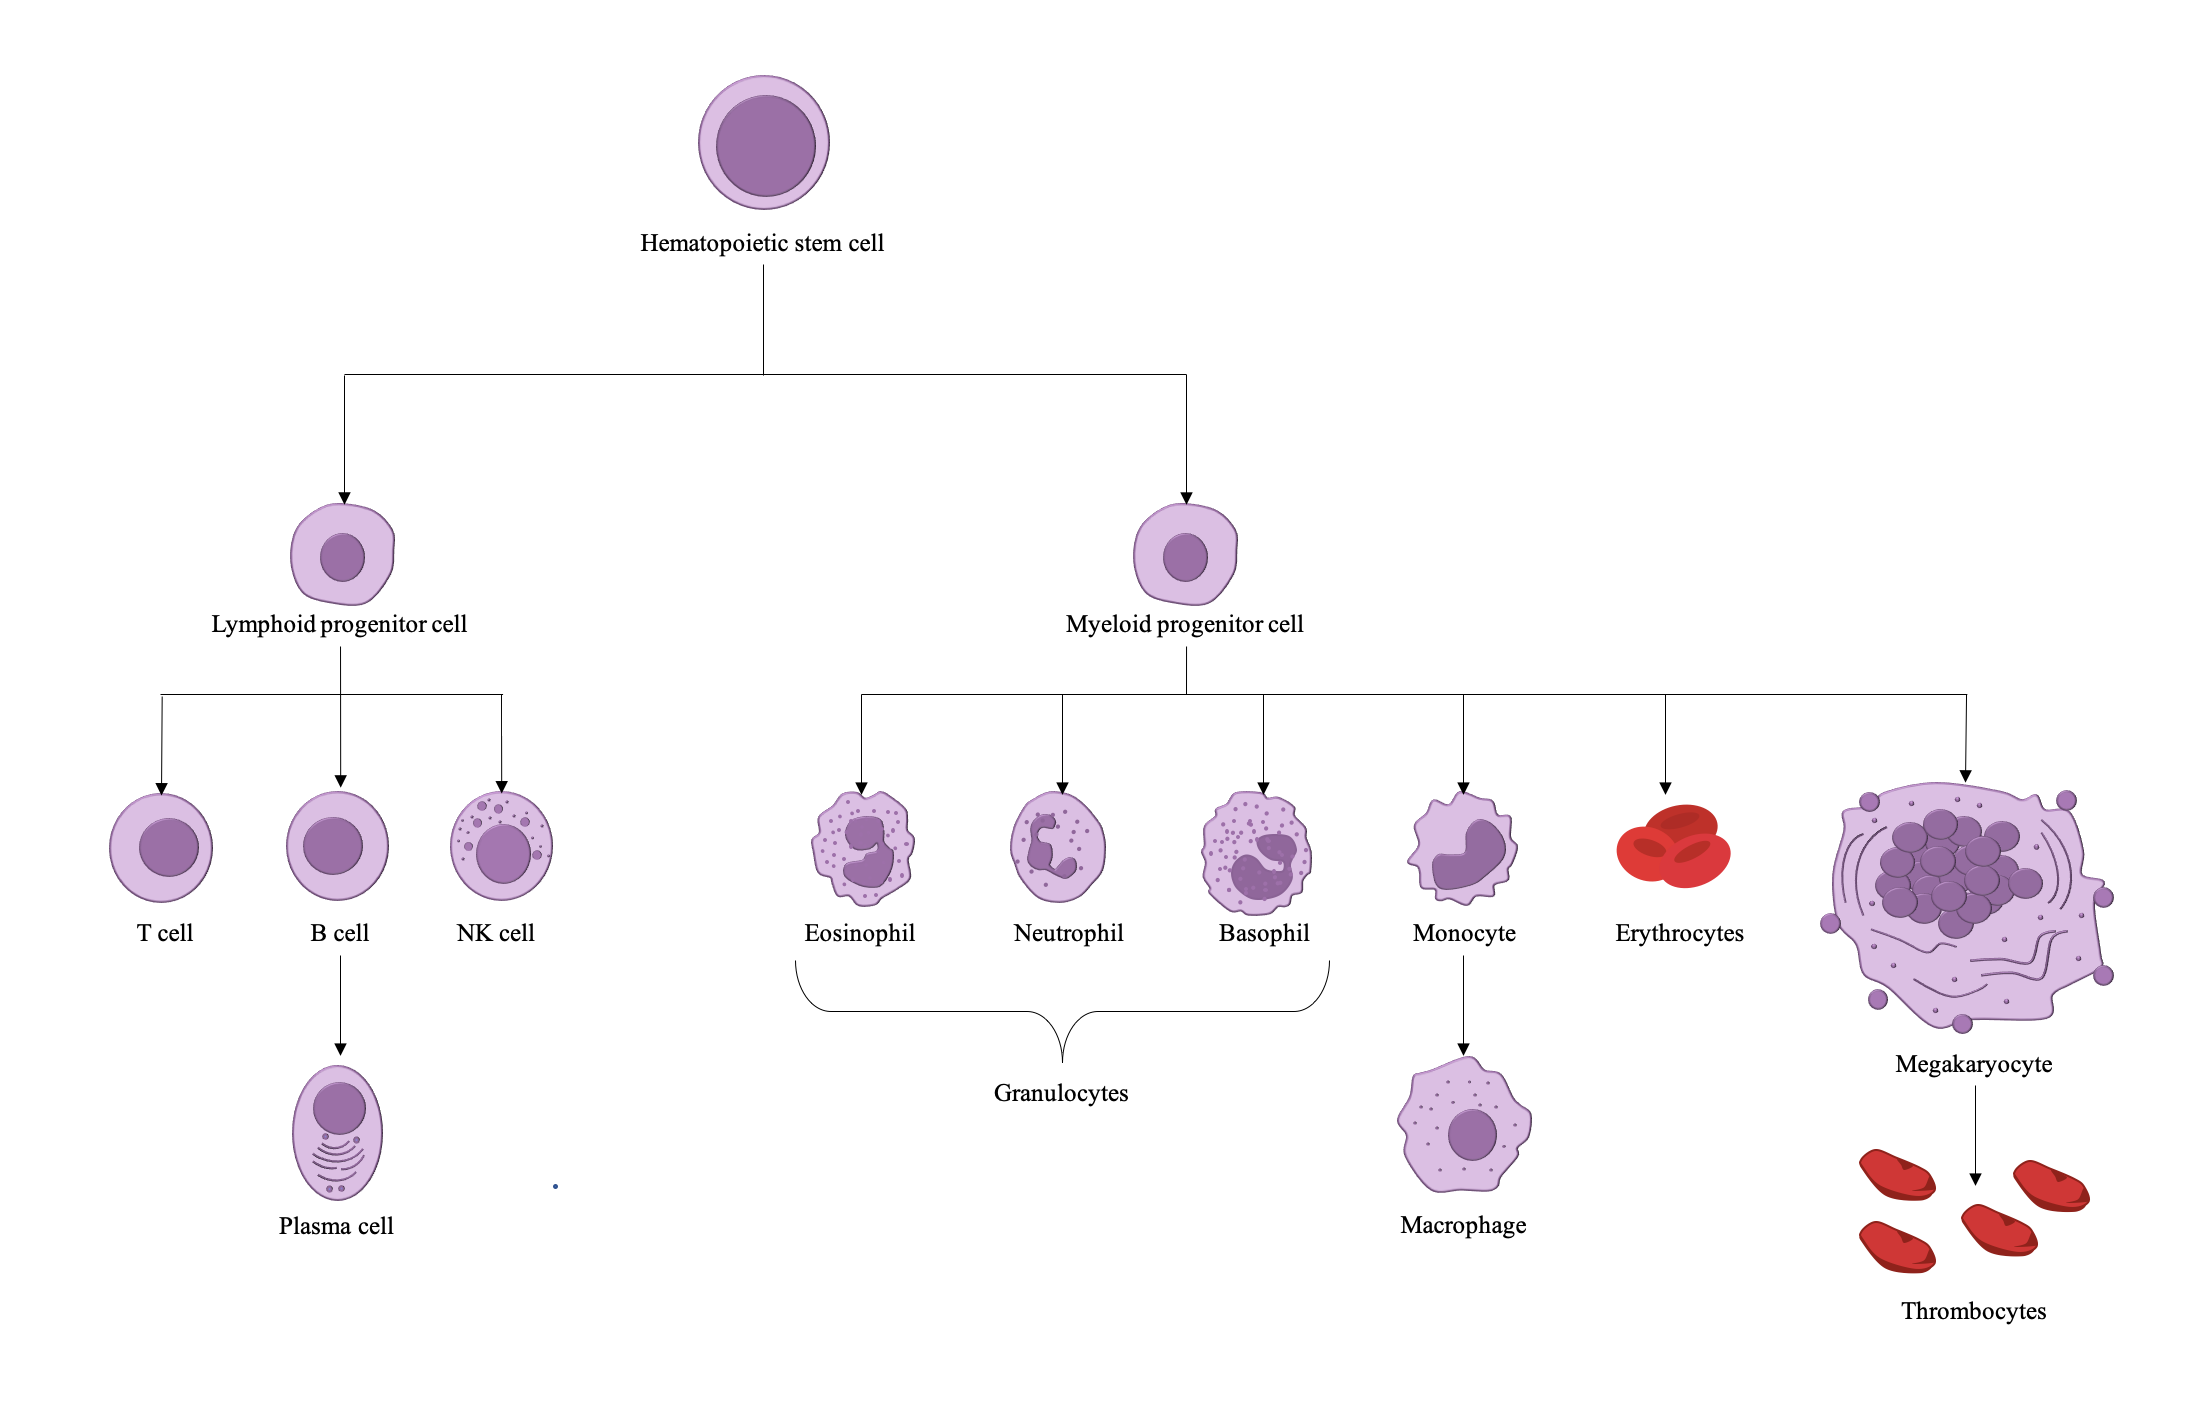
\includegraphics[width=0.7\textwidth]{figures/Introduction/immune_cells.png}
\caption[Hematopoietic system cell differentiation]{Hematopoietic stem cell (HSC) cell differentiation. HSCs divide into myeloid or lymphoid progenitor cells. Dendritic cells and a number of precursor states have been ommitted. }
\label{fig:HSC_differentiation}\end{figure}
%%

Most B cells die in the bone marrow soon after developing, however some will develop in the bone marrow, where initial stages of maturation occur and then migrate to secondary lymphoid organs, such as the spleen.
Within secondary lymphoid organs, numerous critical decisions on B cell fate are made, involving complex transcriptional networks, cell interactions, gene rearrangements, and mutations\cite{roth2014tracking, jourdan2011characterization}.
Upon antigenic-stimulation, naive B cells differentiate into memory B cells or plasma cells.
Terminally differentiated plasma cells are the final effectors of the B cell lineage, each dedicated to secreting large amounts of a single type of antibody.
Plasma cells have an extensive rough endoplasmic reticulum (ER), and have numerous genes involved in immunoglobulin secretion upregulated, including \textit{XBP-1} and \textit{CHOP}\cite{shapiro2004plasma}, to enable the production of copious amounts of antibody.
Plasma cells appear to consist of two distinct categories: short-lived plasma cells, which have life-spans of several months and are located in extrafollicular locales such as in medullary chords of lymph nodes or the red pulp of the spleen, and long-lived plasma cells, which have life-spans of decades and are mainly found in the bone marrow\cite{bortnick2013and, andraud2012living}.



%1
\section{Multiple myeloma}\label{sec:MM}
%2
\subsection{Multiple myeloma cells}
Multiple myeloma is a malignancy of terminally differentiated plasma cells.
It is characterised by aberrant proliferation of clonal, long-lived plasma cells in the bone marrow\cite{anderson2011pathogenesis}.
The large accumulation of MM cells in the bone marrow, crowd out healthy cells.
Under normal conditions, plasma cells produce antibodies that fight infection as part of the adaptive immune system.
However malignant plasma cells (MM cells) produce large amounts of abnormal antibodies that are unable to fight infection, coined `paraproteins' or `M proteins' (Figure \ref{fig:m_spike}).

%% M spike
\begin{figure}
\centering
\includegraphics[width=\textwidth]{figures/Introduction/M_spike.pdf}
\caption[M spike diagram]{Diagram of serum protein electrophoresis (SPEP) for a normal individual and for a multiple myeloma (MM) patient.
Based on their electrical charge, SPEP separates all the proteins in the blood.
A large peak is recorded for albumin (the most abundant protein in the blood), followed by lower levels of the other proteins, grouped into areas labelled $\alpha1$ and $\alpha2$, then a $\beta$ region, and then a $\gamma$ region, which represents where antibodies lie on the graph.
The large quantities of a single type of antibody (M protein) produced by MM cells cause a distinct `M spike' in the antibody protein region of the graph ($\gamma$ region).}
\label{fig:m_spike}
\end{figure}
%%

%2
\subsection{Epidemiology}
Multiple myeloma accounts for 1-2\% of all cancers and has the second highest incidence of hematological malignancies, after non-Hodgkin's lymphoma\cite{international2003criteria}.
MM is rare in individuals under the age of 40, with the average age at time of diagnosis centering around 70\cite{tsang2019multiple, palumbo2011multiple}.
MM is more prevalent in males than females and is around twice as common in black populations than in Caucasian or Asian populations\cite{nhsmyeloma}.
The average incidence rate is approximately 1-6 cases per 100,000 individuals\cite{tsang2019multiple, palumbo2011multiple, teras20162016}, with the highest age-standardised incidence rates in the regions of Australasia, North America, and Western Europe\cite{cowan2018global}.
Five-year survival rate of MM patients is approximately 49\%, whilst approximately a third of MM patients survive ten years or greater\cite{cancerresearchuk, siegel2016cancer}.
%While there have been many successful medicines developed for myeloma, they all suffer from the development of drug resistance.

%2
\subsection{Presentation}
%3
\subsubsection{Precursor states}
All cases of MM are preceded by asymptomatic precursor states, monoclonal gammopathy of unknown significance (MGUS) and smoldering multiple myeloma (SMM).
However, only some patients with SMM or MGUS progress to active MM.

MGUS is a pre-malignant condition where patients have the presence of monoclonal immunoglobulins in their blood or urine, $<$10\% clonal plasma cells in their bone marrow, but lack any myeloma-related end-organ damage\cite{van2018mgus}.
Patients with SMM have between 10 and 60\% clonal plasma cells in their bone marrow, serum monoclonal immunoglobulin of $\ge$3 g/dL, and like MGUS, have no signs of end-organ damage\cite{rajkumar2015smoldering}.
Progression risk of MGUS into symptomatic MM is about 1\% per year, whilst progression risk of SMM to MM is higher, at around 10\% per year for the first 5 years, after which it decreases\cite{korde2011monoclonal, kyle2007clinical}.
%

%3
\subsubsection{Active MM}
There are multiple classifications of active MM.
The International Myeloma Working Group's definition\cite{rajkumar2014international} is as follows:
Greater than 10\% clonal plasma cells located in the bone marrow and one or more myeloma-defining event or biomarker of malignancy.
Myeloma defining events consist of evidence of end-organ damage that can be attributed to the surplus of M protein and clonal plasma cells, namely the CRAB features:
%
% List of myeloma events (CRAB)
\begin{itemize}
  \item Hypercalcemia
    \begin{itemize}
        \item Serum calcium $>$ 1 mg/dL higher than the upper limit of normal, or
        \item Serum calcium $>$ 11 mg/dL
    \end{itemize}
  \item Renal insufficiency
    \begin{itemize}
        \item Creatinine clearance $<$ 40 mL per min, or
        \item Serum creatine $>$ 2 mg/dL
  \end{itemize}
  \item Anemia
    \begin{itemize}
        \item Hemoglobin value of $>$  20 g/L below the lower limit of normal, or
        \item Hemoglobin value $<$ 100 g/L
    \end{itemize}
    \item Bone lesions
      \begin{itemize}
        \item One or more osteolytic lesions on skeletal radiography, CT or PET-CT
        \end{itemize}
\end{itemize}
% End of list
%

Biomarkers of malignancy include greater than or equal to 60\% clonal plasma cells in the bone marrow, an involved:uninvolved serum free light chain ratio greater than or equal to 100, and more than one focal lesion on an MRI study\cite{rajkumar2014international}.

%
It is currently unclear what causes the malignant transformation between precursor states and active MM\@.
However certain factors have been identified as risk factors, including point mutations, a large array of up-regulated transcription factors, and numerous immune events.

\subsection{Treatment of multiple myeloma}\label{subsec:mm_treatment}
Multiple myeloma may be an incurable disease, however it is treatable.
In fact, in the last decade median survival time for newly diagnosed MM patients has almost doubled\cite{kazandjian2016look}.
Novel therapeutic advances have contributed to this improvement (Table \ref{tab:treatment_history}).
Myeloma is usually treated with a combination of drugs, often comprising a corticosteriod, a proteasome inhibitor, and an immunomodulatory drug (IMiD).
A common regimen, approved in the USA, European Union and UK for untreated myeloma is the triplet VRd regimen.
This consists of the proteasome inhibitor bortezomib (brand name Velcade), the IMiD lenalidomide (brand name Revlimid), and the corticosteroid dexamethasone.

% Timeline of treatment options
%% Table for treatment timeline


\begin{table}[h]
\centering
\begin{tabular}{|p{1cm}|p{3cm}|p{8cm}|p{1.3cm}|}
\hline
\textbf{Year} & \textbf{Treatment} & \textbf{Usage} & \textbf{Ref} \\ \hline
1958 & Melphalan & The alkylating agent melphalan was first used in plasma cell myeloma in 1958. & \cite{blokhin1958clinical} \\ \hline
1960s & Corticosteroids & Placebo-controlled double-blind trial of prednisone in multiple myeloma. Combinations of prednisone and melphalan showed an increased survival over melphalan alone. Dexamethasone and prednisone have become a cornerstone in the treatment of multiple myeloma. & \cite{mass1962comparison, alexanian1969treatment} \\ \hline
1980s & Stem-cell transplantations & Numerous successful allogenic and autologous bone marrow transplantations in patients with multiple myeloma &  \cite{mcelwain1983high, osserman1982identical, fefer1986identical, gahrton1987bone}  \\ \hline
2003 & Proteasome inhibitors & Bortezomib, a first-in-class proteasome inhibitor, was first approved by the FDA for use in relapsed and refractory multiple myeloma. In 2008 it was approved for patients with no prior treatment. Carfilzomib was approved in 2012 for advanced MM and later in 2015 for treatment of relapsed MM. The oral proteasome inhibitor, ixazomib, was approved as a combination treatment with lenalidomide and dexamethasone in 2016 for people who have received at least one previous treatment. & \cite{kane2003velcade,richardson2003phase,katsnelson2012next} \\ \hline
2006 & IMiDs & The antitumour activity of thalidomide was demonstrated in 1999, this led to the development of lenalidomide, the first approved immunomodulatory imide drug (IMiD) for use in multiple myeloma. Currently, thalidomide, lenalidomide and pomalidomide are approved for use in multiple myeloma & \cite{singhal1999antitumor,label47revlimid,san2013pomalidomide} \\ \hline
2015 & Monoclonal antibodies & In 2015, daratumumab, an anti-CD38 monoclonal antibody and elotuzumab, an anti-SLAMF7 monoclonal antibody, were approved for MM treatment. & \cite{lokhorst2015targeting,lonial2015elotuzumab} \\ \hline
\end{tabular}
\caption[Timeline of treatment options for multiple myeloma]{Timeline of treatment options for multiple myeloma. Listed by first usage or FDA approval for MM.}
\label{tab:treatment_history}
\end{table}

% https://www.ncbi.nlm.nih.gov/pmc/articles/PMC5282737/
% https://www.ncbi.nlm.nih.gov/pmc/articles/PMC2265446/
% Panobinostat	HDACi
% Liposomal doxorubicin	DNA inter-calator



\subsection{Proteasome inhibitors}
Proteasome inhibitors have contributed greatly to the improved prognosis of MM since their introduction into treatment regimes.
The first-in-class proteasome inhibitor bortezomib (Velcade\textsuperscript{\textregistered}) was approved by the FDA in 2003 as a single-agent for injection of relapsed MM\cite{kane2003velcade}.
Since then it has been approved for use in combination therapies.
Bortezomib in combination with melphalan-prednisone proved to be superior to the previous standard of care for patients ineligible for HDT-ASCT of melphalan-prednisone alone, increasing time until tumour progression\cite{san2008bortezomib}.
The combination of bortezomib, dexamethasone and thalidomide  was also shown to be superior to previous standard of care for patients prior to ASCT\cite{moreau2012proteasome}.
In 2010, bortezomib was approved as a frontline therapy for treatment-naive MM patients.
Since then, two more proteasome inhibitors have been approved, carfilzomib and ixazomib.
Carfilzomib is structurally and mechanistically different to bortezomib and shows activity on bortezomib resistant primary MM cells\cite{moreau2012proteasome}; it is approved for relapsed or refractory MM\@.

\subsubsection{The ubiquitin-proteasome system}
Proteasome inhibitors work by blocking the action of the proteasome in the cell.
Misfolded proteins can be harmful to a cell, so the combined activity of molecular chaperones, which aid in protein folding, and the ubiquitin-proteasome system (UPS), which acts to digest misfolded proteins, is needed to prevent massive protein aggregation.
Unneeded, misfolded or damaged proteins are tagged with lysine-48-linked poly-ubiquitin chains, marking them for degradation by the proteasome (Figure \ref{fig:26s_proteasome_structure}).
The proteasome is sometimes described as a complex `protein destruction machine'.
The proteasome consists of the 20S core particle, a central hollow cylinder, and the 19S regulatory caps associated with each end of the cylinder.
The 19S regulatory caps perform substrate recognition, deubiquitination, unfolding and threading of the protein substrate into the 20S core.
The core is made up of four stacked heptameric ring structures.
The outer rings are responsible for docking to the 19S cap and for acting as a gate to the inner rings. The inner rings consist of seven $\beta$ subunits, containing inward-facing protease active sites for degrading proteins\cite{kleiger2014perilous, alberts2007molecular} (Figures \ref{fig:26s_proteasome_structure} and  \ref{fig:proteasome_beta_subunits}).

 % Proteasome structure diagram
\begin{figure}[ht]
%1
\begin{subfigure}[t]{0.5\textwidth}
    \includegraphics[width=\textwidth]{figures/Introduction/26s_proteasome_serif.jpg}
    \caption{26S proteasome}
    \label{fig:26s_proteasome_structure}
\end{subfigure}
%\medskip
\begin{subfigure}[t]{0.5\textwidth}
    \includegraphics[width=\textwidth]{figures/Introduction/20s_core_beta_subunits_serif.jpg}
    \caption{$\beta$-subunits of an inner ring of the 20S core particle }
    \label{fig:proteasome_beta_subunits}
\end{subfigure}
    \caption[Structure of the proteasome]{Structure of the proteasome. \ref{fig:26s_proteasome_structure} shows the structure of the 26S proteasome, comprised of the 19S regulatory caps and 20S core particle.
    A misfolded protein tagged with a poly-ubiquitin chain is recognised by the 19s regulatory cap, which cleaves the ubiquitins from the protein and threads the protein through to the core, where it is degraded into small peptides.
    The 20S core particle is made up of two outer rings of $\alpha$-subunits and two inner rings of $\beta$-subunits.
    \ref{fig:proteasome_beta_subunits} shows the $\beta$-subunit arrangement in one of the inner rings of the 20s particle.
    $\beta1$ (caspase-like), $\beta2$ (trypsin-like) and $\beta5$ (chymotrypsin-like) are the proteolytically active subunits.
    Proteasome inhibitors are designed to primarily inhibit $\beta5$.}
\label{fig:proteasome_and_beta}
\end{figure}

\subsubsection{Mechanism of action}
Of the seven proteasome $\beta$ subunits, only $\beta1$, $\beta3$ and $\beta5$ are proteolytically active (Figure \ref{fig:proteasome_beta_subunits}). Proteasome inhibitors are designed to target $\beta5$ as it has been shown as the rate limiting protease for proteasomal protein turnover \cite{besse2019proteasome}. Bortezomib reversibly co-inhibits $\beta5$ and $\beta1$ subunits, whilst carfilzomib irreversibly binds to $\beta5$, with greater selectivity than bortezomib, and at higher doses binds to $\beta2$ as well \cite{besse2019proteasome}.


The precise downstream effects of $\beta$ subunit proteasome inhibition are not fully understood, however the unfolded protein response (UPR), NF-$\kappa$B signalling, JNK signalling, apoptotic factors and p53 are thought to be involved in the anti-MM effects \cite{kubiczkova2014proteasome}.
Specifically, the action of the UPR has been demonstrated as an important mechanism in the anti-MM effect of PIs.
MM cells secrete large amounts of monoclonal protein, leading to the rapid accumulation of  misfolded proteins within the endoplasmic-reticulum (ER) lumen.
This results in heightened ER stress, which is compensated by the UPR by reducing global protein translation and up-regulating UPS machinery \cite{wallington2018resistance}.
Therefore, by inhibiting the proteasome, fewer ubiquitin tagged proteins are degraded and more misfolded proteins accumulate in the ER lumen.
ER stress is then further increased, causing the UPR to switch from a homeostatic, pro-survival system to a pro-apoptotic pathway \cite{kubiczkova2014proteasome, wallington2018resistance}.

Another important mechanism for PI is the attenuation of NF-$\kappa$B signalling. I$\kappa$B$\alpha$, a specific endogenous inhibitor of the transcription factor NF$\kappa$B, is a protein degraded by the proteasome.
Inhibition of the proteasome increases levels of I$\kappa$B$\alpha$, thereby abolishing NF$\kappa$B signalling.
NF$\kappa$B is a key transcription factor in many cancers, contributing to overall tumour growth and chemoresistance.
NF$\kappa$B has been shown to promote tumour cell proliferation, anti-apoptotic and angiogenic factors \cite{kale2012molecular}.

\section{Drug resistance in multiple myeloma}
Although PIs are extremely effective at killing MM cells initially, long-term treatment inevitably results in a drug-resistant relapse.
Drug resistance is one of the biggest barriers in the treatment of MM.
Patients follow a pattern of peaks and troughs of treatment cycles, remission and relapse, until all therapies have little effect (Figure \ref{fig:treatment_cycles}).
%% Treatment cycles
\begin{figure}[htb]
\centering
\includegraphics[width=\textwidth]{figures/Introduction/treatment_cycles.pdf}
\caption[MM treatment cycles]{MM treatment cycles and disease progression over time.
All MM patients begin with precursor states Monoclonal Gammopathy of Unknown Significance (MGUS) and/or smoldering multiple myeloma (SMM) prior to a malignant transformation to symptomatic/active MM.
Patients undergo cycles of treatment, remission and relapse until eventually becoming relapsed and refractory (RRMM) and no longer respond to treatment.
}
\label{fig:treatment_cycles}
\end{figure}
%%
In order to overcome resistance and increase overall survival of MM patients, the molecular mechanisms of resistance to proteasome inhibitors needs to be understood.
This  will aid in the design of novel therapies and inform better use of existing therapies.
Previous studies on proteasome drug resistance have been performed and certain mechanisms and genes have been identified.
For example, point mutations have been noted in the \textit{PSMB5} gene (coding for the $\beta5$ subunit of the proteasome), as well as and over-expression of the $\beta5$ subunit \cite{robak2018drug}.
Other upregulated genes have been identified, for example \textit{ABCB1}, coding for P-glycoprotein, responsible for pumping various substrates out of the cell, also referred to as multidrug resistant protein 1.
\textit{XBP1}, involved in the UPR, has been seen to be downregulated in PI resistance \cite{robak2018drug}.
Although many genes have been identified to be differentially expressed in drug resistant MM, the mechanism is not fully elucidated and further research is imperative in the progression of treatment for multiple myeloma.

Another avenue to increase MM survival, would be to identify novel therapeutics effective against MM, which are capable of overcoming acquired anti-cancer drug resistance.
By increasing the arsenal of drugs available to treat MM, the time until patients become refractory and no longer respond to treatment could be prolonged.
Therapeutics with a novel mechanism of action are likely to be more effective for MM patients who have undergone several treatment cycles than drugs belonging to the same class as drugs they have previously been treated with.
Novel therapeutics would have less overlap of mechanism of action with existing drugs, therefore there would be less cross-resistance.

%
\afterpage{\clearpage} % flush out floats before this. Very different section
%
\section{Transcriptomics, proteomics and epigenomics}
It has been shown that changes in the genome, transcriptome, epigenome and proteome all contribute to disease progression and drug resistance in MM.
Therefore, to sufficiently investigate the multiple layers driving MM and to assess the effectiveness of new therapeutics, a multi-omics approach must be employed.

\subsection{DNA and the genome}\label{subsec:dna}
The genome is the genetic material of an organism, it consists of deoxyribonucleic acid (DNA).
DNA consists of two polynucleotide chains (or strands), running anti-parallel to each other, held together in a double helix structure by hydrogen bonds.
Nucleotides are composed of a five-carbon sugar (deoxyribose for DNA), attached to one or more phosphate group (a single phosphate group in the case of DNA) and a nitrogenous base.
Nucleotides are covalently linked to form an alternating sugar-phosphate backbone, with bases extending from each sugar towards the inside of the double helix.
Nucleotides contain four different types of bases: adenine (A), cytosine (C), guanine (G) and thymine (T).
The two DNA chains are held together by hydrogen bonds via complementary base pairing between the bases of the strands, A pairing with T and G pairing with C\@.
Often sections of DNA are denoted as their sequence of A, C, T and Gs (in order reading from the 5' to 3' direction).

Every individual has approximately 6 billion base pairs of DNA per cell, which would amount to about 2 metres of DNA if laid end-to-end.
The nucleus of a human cell is approximately 6\si{\micro\meter} in diameter, therefore chromosomal DNA must be folded tightly to fit.
DNA packaging is a complex task involving numerous speciliased proteins.
Negatively charged DNA is complexed with an octomer of positively charged proteins called histones to form nucleosomes.
The histone core is made up of eight subunits, two copies of H2A, H2B, H3 and H4 subunits.
DNA wraps tightly around the histone core 1.65 times.
Linker DNA connects adjacent nucleosomes, to resemble `beads on a string'.
Nucleosomes fold tightly to form 30\si{\nm} chromatin fibre, which in turns forms loops averaging 300\si{\nm} in length.
This fibre is folded and compressed again to form fiber 250\si{\nm} in width with loops of 700\si{\nm} in length.
Tight coiling of this fiber forms the single chromatids of chromosomes \cite{annunziato2008dna, alberts2002chromosomal}.
Human cells contain 23 pairs of chromosomes.

% DNA structure and packaging
\begin{figure}[htb]
%1
\begin{subfigure}[t]{0.5\textwidth}
    \includegraphics[width=\textwidth]{figures/Introduction/nucleotides_dna_helix.png}
    \caption{Nucleotide and DNA double helix structure}
    \label{fig:base_pairs}
\end{subfigure}
%\medskip
\begin{subfigure}[t]{0.5\textwidth}
    \includegraphics[width=\textwidth]{figures/Introduction/dna_packaging.png}
    \caption{DNA packaging}
    \label{fig:DNA_packaging}
\end{subfigure}
    \caption[DNA stucture and packaging.]{\ref{fig:base_pairs} shows the DNA nucleotides and the DNA double helix structure.
    DNA consists of two polynucleotide chains.
    Nucleotides are covalently linked to one another, forming a sugar-phosphate backbone.
    They contain one of four bases adenine (A), cytosine (C), guanine (G) and thymine (T).
    DNA strands are held together by hydrogen bonds between complementary base pairs, A pairing with T and G pairing with C\@.
    Sections of DNA are are often read by their sequence of bases from the 5' direction to the 3' direction.
    \ref{fig:DNA_packaging} shows how chromosomal DNA is packaged in the cell.
    DNA wraps 1.65 times around an octomer of histone proteins, to form a stucture called a nucleosome.
    Nucleosomes are linked by linker DNA to form a structure that resembles `beads on a string'.
    Nucleosomes fold to create chromatin fiber.
    This is turn forms loops and coils tighter and tighter until it makes up the single chromatids of chromosomes.
    \\\hspace{\textwidth}Created with BioRender.com.
    }
\label{fig:DNA_structure_packaging}
\end{figure}

The complete genome is made up of coding DNA (genes), non-coding DNA, as well as mitochondrial DNA and ribosomal DNA\@.
An alteration in the nucleotide sequence of the genome is called a mutation.
There are a number of types of mutations, including insertions, deletions, inversions, substitutions and duplications.
A technique called whole genome sequencing (WGS) can be used to determine the sequence of nucleotides in an individual's DNA and therefore it can be used to determine any variations in the genome.
% However the technique is expensive and many experiments are interested in coding DNA only, so perform RNA-seq to look at the transcriptome instead.

% Diagram double helix with bases in the middle. Then one of sequence of ACTG etc.
% Diagram of DNA genes transcribed to RNA then translated to proteins (pg 301 of textbook is good example)

\subsection{The epigenome}
Epigenetics is the study of any heritable phenotypic changes that do not involve alterations of the DNA sequence itself.
These changes occur at the chromatin level.
Epigenetic changes include histone modifications, DNA methylation and chromatin remodelling.
%These epigenetic changes are described in more detail below.

DNA methylation is the addition of methyl groups to the C5 position of cytosines in DNA.
This happens extensively at CpG sites (cytosine followed by a guanine).
Stretches of DNA with a high CpG ratio (CpG islands) are often found in the promoter region of genes.
Increased DNA methylation at CpG islands results in transcriptional silencing of those genes.
Genome wide DNA methylation is often examined using DNA-methylation-seq or DNA methylation microarrays.

DNA wraps tightly around histones (section \ref{subsec:dna}), they contribute to the tight packaging of DNA.
Histone modifications are post-translational modifications.
They include methylation, acetylation, phosphorylation, ubiquitination and sumoylation.
Histone modifications affect transcriptional activity either by directly influencing the structure of chromatin and DNA accessibility or by regulating binding of effector molecules to `read' histone marks to mediate downstream biological effects.
Histone modifications also regulate DNA processes, such as repair, replication and recombination \cite{ bannister2011regulation}.
Chip-seq can be used to investigate and measure various post-translational histone modifications.

Chromatin remodelling is the process of modifying chromatin architecture to regulate the accessibility of DNA.
Gene expression is regulated by allowing certain gene regions better access to transcription machinery.
This is achieved by ATP-dependent chromatin-remodelling complexes moving, ejecting or restructuring nucleosomes.
ATAC-seq can be used to identify accessible DNA regions.


\subsection{The transcriptome}
Transcription is the first of many steps in gene expression.
During transcription, the enzyme RNA polymerase reads a DNA sequence and produces an anti-parallel, complementary ribonucleic acid (RNA) strand.
The transcriptome is the set of all RNA transcripts of an individual.
RNA is a nucleic acid similar to DNA. Like DNA it has a sugar-phosphate backbone and 4 different types of bases attached to each sugar.
However, unlike DNA, RNA is single-stranded, it contains the sugar ribose in place of deoxyribose, and the nucleotide uracil (U) inplace of thymine (T).

Despite the chemical differences between DNA and RNA, they are essentially written in the `same language' and one-to-one mapping of nucleotides can be performed.
Transcription begins with the unwinding and opening of a small part of the DNA double helix, so bases are exposed.
One strand of DNA acts as a template and the RNA chain is formed by complementary base pairing with the template.
RNA polymerases catalyse the reaction of forming phosphodiester bonds between nucleotides, forming the RNA chain.
The RNA polymerase moves stepwise along the DNA chain, unwinding the chain just ahead exposing a new region of the template strand.
Just behind the region where ribonucleotides are being added, the DNA helix reforms.

The genes in a cell's DNA that specify the amino acid sequence and result in protein synthesis are called messenger RNA (mRNA) molecules.
Genes that produce the RNA molecule itself are called non-coding RNAs, because they do not code for proteins.
There are many other types of RNA, such as transfer RNA (tRNA), ribosomal RNA (rRNA) and micro RNA (miRNA).

Traditionally microarrays were used to measure gene expression.
Now RNA-seq (outlined in section  \ref{subsec:rna-seq-intro}) is more commonly used study to gene expression and the transcriptome.
Depending on the library preparation, different types of RNAs can be selected for or excluded, to study different RNA molecules.

\subsection{The proteome}\label{subsec:translation}
The proteome is the entire set of proteins that is or can be expressed by an organism.
mRNAs are translated into protein molecules.
mRNA is made up of only four different nucleotides, but proteins are made up of 20 amino acids, therefore a direct one-to-one function matching nucleotides to amino acids is impossible.
Instead, the sequence of mRNA is read in groups of three consecutive nucleotides, called a codon.
The three positions of a codon, and each position with four possible base options (A, C, U and G), gives a total of 64 different permutations (i.e. 4\textsuperscript{3}).
Therefore, some combinations map to the same amino acid (many-to-one function), or signal to terminate translation of the current protein, named a stop codon.
This genetic code directs the translation from mRNA to protein.
Translation takes place in the ribosome.

Codons on mRNA do not directly recognize their given amino acid, they require tRNA molecules that bind to both the codon on mRNA and the correct amino acid.
tRNAs possess an anticodon, a set of three nucleotides complementary to a given codon.
Firstly, tRNAs are coupled to their cognate amino acid.
This reaction is catalysed by aminoacyl-tRNA synthetase (aaRS) enzymes.
aaRSs attach amino acids to the 3' end of tRNA.
Most cells have a specific aaRS for each amino acid.
Once the tRNA is charged with the correct amino acid, the tRNA molecule binds to its complementary codon on mRNA.
Subsequent aminoacylated tRNA molecules bind to mRNA codons.
A polypeptide chain grows by stepwise addition of amino acid to the C-terminal end.
The formation of the new peptide bond between amino acids releases the tRNA molecule.
The peptide chain grows until a stop codon is reached and synthesis of the current protein is complete.

Protein translation is partly regulated by availability of mRNAs, but it also depends on other factors such as RNA silencing and post-transcriptional modifications.
Proteins have a large array of functions, such as transporting small molecules, catalysing reactions, cell-cell signalling and providing structural support.

Proteomics is the study of the proteome.
CyTOF and LC-MS/MS are techniques often employed to examine the proteome. %(section \ref{subsec:cytof-intro} and section \ref{subsec:lcmsms-intro}).

\subsection{Sequencing}
DNA is often referred to as the `genetic master code', therefore the ability to decode the order of nucelic acids has been seen as a highly desirable feat since its discovery.
Sequencing is the process of determining the sequence of nucleotides of nucleic acid residues.
Over the last half-century, large numbers of researchers and vast sums of money have been applied to facilitate the techniques and technologies to decode DNA and RNA molecules' nucleotide sequence \cite{heather2016sequence}.
Over this time, massive technological innovations have been developed.
The most commonly used `first-generation' DNA-sequencing technology, Sanger sequencing, was developed in 1977 \cite{sanger1977dna}.
In Sanger sequencing, or the `chain termination method', chain-termination PCR is performed with a mix of regular nucleotides (deoxynucleotide triphosphates; dNTPs) and fluorescently-labelled, chain-terminating dNTPs (dideoxynucleotide triphosphates; ddNTPs), using the DNA of interest as a template.
During the extension step of PCR, when DNA polymerase incorporates a ddNTP randomly, extension ceases.
This creates greater than a million copies of the DNA sequence of interest, all terminated at random lengths by the ddNTPs.
Capillary gel electrophoresis is then used to separate the extension products by size.
The gel is then read to determine the sequence.
By reading the gel bands from smallest to largest, the 5' to 3' sequence of the original DNA strand can be inferred.
Sanger sequencing was used by the Human Genome Project, an international research effort to determine the DNA sequence of the entire human genome \cite{pennisi2001human}.
The whole project took approximately 13 years to complete, and was reported to have cost \$3 billion.

Sanger sequencing dominated the sequencing world for over 30 years, until the advent of `Next-generation sequencing' (NGS; now being dubbed `second-generation sequencing', with the advent of newer technologies).
NGS differs from its predecessors in that it is highly scalable and massively parallel.
With NGS you can rapidly sequence the entire human genome in one day, for just under \$5000.
It is quicker and cheaper than traditional Sanger sequencing, and has progressed data output from the kilobase range up to potentially multiple terabases per run.
Today, the largest and most commonly used NGS sequencing technology platform is Illumina, who own around 80\% of the global sequencing market.
NGS can be used to study the transcriptome, using RNA-seq techniques (Section \ref{subsec:rna-seq-intro}); the epigenome, using techniques such as ChIP-seq or ATAC-seq; or the genome using techniques such as whole genome sequencing (WGS).

Recently, long-read technologies are becoming more prominent in the sequencing field.
Illumina short-read sequencing limits read length to between 50 and 300 base pairs (bp)\@.
This read length is too short to detect more than 70\% of human genome structural variation.
Moreover, some of the most mutation-prone regions of the genome are inaccessible due to repeating or GC-heavy content, limiting sequence coverage and leaving large regions of the genome critically understudied \cite{logsdon2020long}.
Long-read technologies are capable of generating continuous sequences ranging from 10 kilobases to several megabases, enabling the sequencing of full-length transcripts.
The two main emerging long-read technologies are PacBio single-molecule real-time (SMRT) sequencing\cite{wenger2019accurate} and Oxford Nanopore Technologies (ONT) sequencing\cite{ip2015minion, jain2016oxford}, together marking the birth of `third-generation sequencing' (TGS).
Both PacBio and ONT sequencing sequence single DNA molecules, rather than a pool of PCR-amplified fragments.
PacBio sequencing employs a sequencing-by-synthesis strategy (similar to Illumina sequencing), with circular DNA templates to improve accuracy.
ONT sequences a native linear single-stranded DNA molecule by measuring current changes as bases are threaded through a nanopore \cite{weirather2017comprehensive}.
Whilst TGS technologies have the advantage of longer read length, the methods are also plagued by higher base-calling error rates and lower throughput than NGS technologies \cite{weirather2017comprehensive, philpott2021nanopore}.
Therefore, this makes applying TGS to single-cell RNA-seq especially challenging.
Due to the lower through-put, fewer cells can be reported on at a comparable read-depth to NGS technologies;
and due to the high base-calling error rate, inaccurate cellular and molecular barcode assignment can complicate associating mRNA reads with their cell of origin.

\subsection{RNA-seq}\label{subsec:rna-seq-intro}
Most modern RNA sequencing (RNA-seq) implements NGS technology to analyse RNA across the transcriptome of a biological sample and allows for the quantification of gene expression.

\subsubsection{Bulk RNA-seq}
Bulk RNA-seq measures the average expression across a sample.
Creating a bulk RNA-seq library involves isolating RNA from a biological sample, filtering for a specific type of RNA (most commonly mRNA), fragmentation of RNA into fragments, reverse transcription of the fragments to generate a complementary DNA (cDNA) library, end repair and adaptor ligation of the cDNA library, followed by PCR amplification ready for sequencing.

%% Diagram of bulk RNA-seq
\begin{figure}[ht]
\centering
\includegraphics[width=0.8\textwidth]{figures/Introduction/bulk_rna_library_prep_diagram_alternate.png}
\caption[Bulk RNA-seq outline]{Outline of bulk RNA-sequencing library prep.
Cells are lysed and RNA is extracted.
The specific RNA of interest is selected and enriched, for example selecting for mRNA using polyA selection or ribo-depletion.
The mRNA is fragmented into smaller pieces of RNA.
First and second stranded cDNA are reverse transcribed from the RNA fragments using random primers.
The ends of the cDNA are repaired and dAMP (dA) tails are added to the 3' end of the DNA.
Adaptors are ligated to the 3' and 5' end of the cDNA.
These adaptors contain complementary sequences that allow the fragments to hybridize to the flow cell during sequencing.
Universal (P5/i5) and index (P7/i7) primers are added to the adaptor ligated DNA.
The libraries are then amplified using PCR and cleaned-up, ready for sequencing.
}
\label{fig:bulk_diagram}\end{figure}
%%

\subsubsection{Single-cell RNA-seq}
Single-cell RNA-seq (scRNA-seq) measures gene expression for each individual cell across a population of cells and therefore provides information on clonal diversity that may be lost when pooling cells into bulk samples.
Since its inception in 2009\cite{tang2009mrna}, there have been numerous scRNA-seq techniques developed, such as SMART-seq2\cite{picelli2013smart}, Drop-seq\cite{macosko2015highly}, STRT\cite{islam2011characterization}, scCOLOR-seq\cite{philpott2021nanopore} and inDrops\cite{klein2015droplet}.
scRNA-seq library preparation shares many steps with bulk RNA-seq workflow, however preliminary steps are required to isolate single cells and barcode reads that originated from the cell.
%% Diagram of drop-seq
\begin{figure}[hb]
\centering
\includegraphics[width=0.7\textwidth]{figures/Introduction/drop_seq.png}
\caption[Drop-seq schematic]{Outline of Drop-seq, a droplet-based scRNA-seq method.
A microfluidic device combines two aqueous flows, one containing cells and the other containing barcoded primer beads suspended in lysis buffer.
The two aqueous channels flow across an oil channel to form aqueous droplets surrounded by oil.
Relatively few droplets contain both a cell and a bead.
Following droplet formation, the cell is lysed and its mRNAs are released, which then hybridise to the primers on the bead surface.
A reagent is added to break up the droplets and the beads are collected and washed.
The mRNAs are reverse-transcribed into cDNAs, generating a set of ``STAMPS'' (single-cell transcriptomes attached to microparticles) and template switching is used to introduce a PCR handle.
The barcoded STAMPS can then be amplified using PCR.}
\label{fig:dropseq}\end{figure}
%%
For droplet-based scRNA-seq (dscRNA-seq) methods, single cells are isolated using microfluidic devices by individually encapsulating them in aqueous droplets contained in oil.
Below, a dscRNA-seq method, Drop-seq, is outlined (Figure \ref{fig:dropseq}).


% \subsection{ATAC-seq}

%\subsection{ChIP-Seq}
%Chromatin immunoprecipitation sequencing (ChIP-seq) is used to analyse protein interactions with DNA.
%At a base-pair resolution, it is used to map DNA-binding proteins and histone modifications.
%Therefore ChIP-seq is often used to determine the the mechanisms of gene regulation of transcription factors, and to study epigenetic mechanisms in detail.
%It utilises NGS to identify biding sites of DNA-associated proteins, therefore it is often used to determine the mechanisms of transcription factors or chromatin-associated proteins, influencing gene expression.


%\subsection{CyTOF}\label{subsec:cytof-intro}


%\subsection{Liquid chromatography with tandem mass spectrometry}\label{subsec:lcmsms-intro}
%Liquid chromatography with tandem mass spectrometry (LC-MS/MS) based proteomics is a popular analytical technique to measure the protein abundance of a sample.
%The general steps for LC-MS/MS-based proteomics include: cell lysis, protein extraction, protein digestion using an enzyme to cleave proteins into peptides, peptide purification, and analysis by mass spectrometry.
%The resultant data includes mass and charge (m/z) information and peak intensities.
%Software is then employed which performs database searches and calculates the most likely peptide for each peak.
%From this data, protein abundance can then be calculated and normalised.

%LC-MS/MS-based proteomics can also be used to search for specific proteins within the proteome.
%For example, immobilized metal affinity chromatography (IMAC) can be used to enrich for phosphorylated peptides (phosphoproteomics), and anti-ubiquitin antibodies can be used to enrich for ubiquitinated peptides (ubiquitinomics).

%\section{Summary}

\section{Thesis aims and chapter outline}
This thesis aims to identify novel therapeutics with anti-MM properties, capable of overcoming acquired drug resistance in MM\@.

\noindent
Chapter \ref{ch:1-intro}: General introduction of the adaptive immune system, multiple myeloma (MM) and treatment of MM, as well as an introduction into the multiple layers of information underpinning life: the genome, transcriptome, epigenome and proteome, and the different multi-omic techniques that can be employed to investigate them.

\noindent
Chapter \ref{ch:2-litreview}: Literature review introducing aminoacyl-tRNA synthetases (aaRS), the roles they play in disease and therapeutics targeting aaRSs, focusing on the prolyl-tRNA synthetase inhibitor, Halofuginone (HF) and its applications, particularly in multiple myeloma.

\noindent
Chapter \ref{ch:3-methods}: Experimental materials and methodology used in this work.

\noindent
Chapter \ref{ch:4-Pipelines}: Outline of computational methods generated to support experimental work and benchmark validations of their effectiveness.

\noindent
Chapter \ref{ch:5-bulk}: Investigation of the use of ProRS inhibitors in PI-sensitive and PI-resistant MM cell lines.
Bulk-RNA seq is employed and the transcriptional landscape following ProRS treatment is characterised.

\noindent
Chapter \ref{ch:6-sc}: Exploration of ProRS inhibitor treatment of primary BM samples from MM patients at the single cell level.
Their effectiveness against newly-diagnosed and relapsed MM patient tissue is investigated.

\chapter{\label{ch:2-litreview}Aminoacyl tRNA synthetases and Halofuginone}

\section{Introduction}
Aminoacyl tRNA synthetases (aaRS) are a highly-conserved family of enzymes, responsible for ``charging'' tRNAs with their cognate amino acid.
Human cytoplasmic aaRSs are either ``free'' as individual species or bound in a macromolecular complex, comprised of eight aaRSs and three auxiliary proteins, known as the multi-tRNA synthetase complex (MSC).
On top of their canonical enzymatic role, aaRSs also engage in non-enzymatic functions in numerous pathways, including angiogenesis, inflammation and metabolism.
Often species are released from the MSC to regulate these non-canonical activities.
aaRSs have been shown to involved in numerous diseases, including cancer.
Initially, due to their high fidelity and complex evolution over millennia, aaRSs were seen as an attractive drug target for antimicrobials, to enable specifically targeting microbial aaRSs with minimal effects on human cells.
The mechanism of action of Febrifugine (FF), a quinazoline alkaloid that has long been used as an antimalarial remedy, has recently been revealed; it acts as a competitive inhibitor of ProRS (part of the bifunctional glutamyl-prolyl-tRNA synthetase enzyme; EPRS), responsible for charging tRNA\textsuperscript{pro} with proline.
Although it has potent antimalarial effects, Febrifugine exhibits high liver and gastrointestinal (GI) toxicity, so cannot be used as a widespread drug, therefore several analogues of Febrifugine were developed in the hope of minimizing toxicity to the host`s cells.
One such analogue, Halofuginone (HF) was synthesized and was shown to have the most potent antimalarial properties of all the derivatives, with lower toxicity to the host than Febrifugine, but still some liver toxicity and GI side effects remain.
Halofuginone has been applied to and showed promise in many other non-parasitic diseases too.
It has received orphan drug status for scleroderma and HIV-Related Kaposi's Sarcoma.
Recently, Halofuginone`s application in various cancers has become of great interest, including but not limited to: metastatic brain tumours, bladder carcinomas, prostate cancer, renal carcinomas, hepatocellular carcinomas, lung cancer, breast cancer and multiple myeloma.


This review will introduce the structure and function of aminoacyl tRNA synthetases, provide an insight into their role in pathology and potential as therapeutic targets.
EPRS1 and its inhibitors will be the primary focus, and exploring...

\section{Function and structure of aminoacyl tRNA synthetases}

Aminoacyl tRNA synthetases (aaRS) are an ancient family of ubiquitous enzymes, conserved across three major domains of life (but not present in viruses).
They can be traced back prior to the ``Last Universal Common Ancestor'' (LUCA) \cite{de2020evolution}.
aaRSs are essential for protein biosynthesis, and catalyse the first step in translation (see section \ref{subsec:translation}).
aaRSs catalyse the charging of tRNAs with their cognate amino acid.
This is a two-step process.
Firstly, aaRSs catalyse the formation of an aminoacyl-adenylate (activated amino acid) from their corresponding amino acid and an ATP molecule, releasing an inorganic pyrophosphate.
Next, aaRSs catalyse the reaction between the aminoacyl-adenylate and their cognate tRNA to release an AMP molecule and generate an aminoacyl (charged)-tRNA, ready to be used by the ribosome to decode mRNA (see equation \ref{eqn:aminoacyl}).
An example of this process would be prolyl-tRNA synthetase (abbreviated to ProRS) charging tRNA\textsuperscript{pro} with proline.

\begin{equation}\label{eqn:aminoacyl}
\begin{gathered}
aa + ATP \rightleftharpoons  aa.AMP + PPi \\
aa.AMP + tRNA^{aa} \longrightarrow  aa.tRNA^{aa} + AMP
\end{gathered}
\end{equation}

Eukaryotes have 20 cytoplasmic aaRS and 20 nuclear-encoded mitochondrial aaRS.
These are localised in distinct cellular compartments.
aaRSs are often denoted by their one letter amino acid symbol, followed by ARS and either 1 (indicating they are cytoplasmic) or 2 (indicating they are mitochondrial), for example PARS1 for cytoplasmic ProRS.
This review will focus on cytoplasmic aaRS enzymes.
aaRS can be divided into two distinct classes based on the structure of the fold of their catalytic domains.
Class I aaRS enzymes are functional monomers that contain a dinucleotide or Rossman fold (RF) of alternating alpha-helices and parallel beta-sheets.
This fold is where ATP and amino-acid binding takes place and therefore facilitates the aminoacylation reaction.
The active site of class I aaRS is marked by the signature motifs ``HIGH'' (His-Ile-Gly-His) and ``KMSKS'' (Lys-Met-Ser-Lys-Ser).
Within the first half of the RF the HIGH motif helps to correctly position the adenine base of ATP and interacts with the phosphates.
The second K of the KMSKS motif is thought to be involved in stabilising the transition state for the primary step of aminoacylation \cite{newberry2002structural}.
Amino acid recognition and binding takes place in the catalytic site when the KMSKS motif is open.
The KMSKS loop closes after the aaRS binds ATP and the aminoacyl-adenylate is formed \cite{kwon2019aminoacyl}.


Class II aaRS enzymes are functional dimers or tetramers with an uncommon catalytic core, comprising seven anti-parallel beta-sheets, flanked by alpha-helices.
Class II aaRS enzymes are defined by three conserved sequence motifs.
Motif 1 is located at the interface of the dimer and enables oligomerization.
Motifs 2 and 3 comprise part of the aminoacylation active site and facilitate amino acid/ ATP binding and adenylate formation.
Motif 3 binds ATP, and motif 2 is involved in coupling ATP and the amino acid and then transferring the amino acid to the 3`-tRNA \cite{kwon2019aminoacyl}.
The distinct active-site structures of class I and II enzymes confer markedly different binding mechanisms for the aminoacylation reaction.
For example, class I aaRSs bind the tRNA acceptor stem via the minor groove side and bind ATP in an extended conformation, whilst class II aaRSs bind the tRNA acceptor stem from the major groove side and bind ATP in a bent conformation.
The two classes of aaRSs split the twenty amino acids into two groups.
Val, Leu, Ile, Met, Glu, Gln, Trp, Tyr, Arg and Cys are activated by their cognate class I aaRS; and Gly, Pro, Ala, Thr, Ser, Hist, Asp, Asm, Lys and Phe are activated by their cognate class II aaRS.
Class I and class II can be further divided into different sub-groups, however that is beyond the scope of this review.
The structural diversity of aaRSs is likely attributable to the need to exclude similar non-cognate amino acids and to discriminate the correct tRNA isoacceptor.

Both class I and class II aaRSs are multi-domain proteins- in addition to their catalytic domains, they include other domains such as their anti-codon recognition domain or an editing domain.
The editing domain found in some aaRSs is to ensure that the essential step of aminoacylation in protein biosynthesis is as accurate as possible, so incorrect amino acids can be removed from aminoacyl-adenylates or mischarged tRNAs \cite{kwon2019aminoacyl}.
Theoretically, it was estimated that mistranslation rate should be approximately 1 in 200 for amino acids differing by just a methyl group (such as valine and isoleucine) \cite{pauling1958festschrift}, however in-vivo work demonstrated that the error frequency is closer to 3 in 10,000 (approximately 1 in 3000) \cite{loftfield1972frequency}.
This suggested the existence of proof-reading capabilities of aaRSs, to account for the difference between observed and predicted error rates.
Editing capability has since been shown to be of high functional importance to some aaRSs.
For example, a study in mice in which there was a missense in the editing domain of AlaRS.
The impaired proof reading activity of the enzyme lead to an accumulation of misfolded proteins, resulting in the activation of the unfolded protein response and substantial neurodegeneration \cite{lee2006editing}.
Not all aaRSs possess editing activity, only about half do, however the high specificity of the active site of those aaRSs is enough to alleviate proofreading need.

\subsection{Multi-tRNA synthetase complexes}
Higher eukaryotes contain macromolecular complexes, which consist of nine enzymes and three auxiliary proteins, known as multi-tRNA synthetase complexes (MSC).
The 11 cytoplasmic aaRSs not located in the MSC remain free as individual species.
The nine cytoplasmic aaRS enzymes of the MSC are GluRS (EARS1), ProRS (PARS1), IsoRS (IARS1), MetRS (MARS1), GlnRS (QARS1), LysRS (KARS1), ArgRS (RARS1), AspRS (DARS1), LeuRS (LARS1).
GluRS and ProRS are covalently fused via triple repeats of WHEP domains to form a bifunctional enzyme, EPRS1.
The non-enzyme component of the MSC consists of three aminoacyl-tRNA synthetase-interacting multifunctional proteins (AIMP), AIMP1, AIMP2 and AIMP3.
Human MSCs contain more class II aaRS enzymes than other species, namely DARS1, KARS1, and PARS1, they also contain more auxiliary proteins.
Human MSC components have several additional domains or motifs (Figure \ref{fig:MSC}A), for instance GST-homology domains in EPRS, MetRS, AIMP1 and 2, and WHEP domains in EPRS and MetRS \cite{kim2019evolution, khan20203, kim2020structures}.

The structure of human MSC has not been fully elucidated, however some sub MSC-complex structures have been revealed.
LysRS forms a homodimer and is anchored to the N-terminal peptide region of AIMP2 within the main body of the MSC.
MetRS, AIMP3, EPRS1 and AIMP2 are compactly linked through their GST-homology domains.
ArgRS, GlnRS and AIMP1 assemble into a heterotrimeric complex \cite{kim2019evolution, khan20203, kim2020structures}.
A proposed bisymmetrical model of the human MSC, via homodimerization of AspRS and ProRS, is shown in Figure \ref{fig:MSC}B, based on subcomplex and interaction data \cite{cho2015assembly, kaminska2009dissection, mirande2017aminoacyl}.
This hypothesis proposes that the MSC is a super-complex of two identical, symmetrically arranged subunits (symmetrical along the y-axis in Figure \ref{fig:MSC}B), each containing one copy of the constituent elements, except for LysRS which is present as a dimer in each subunit.

%% Diagram of MSC
\begin{figure}[htb]
\centering
\includegraphics[width=0.6\textwidth]{figures/lit_review/MSC_structure.jpg}
\caption[Multi-tRNA synthetase structure]{The human multi-tRNA synthetase (MSC) and its components.
\textbf{A)} The domains of the aminoacyl tRNA synthetases and auxiliary proteins (AIMP1, 2 and 3) making up the human multi-tRNA synthetase (MSC).
The bifunctional enzyme EPRS1 is made up of the class 1 enzyme GluRS and class II enzyme ProRS (dimer) covalently linked by three WHEP domains.
\textbf{B)} Cartoon representation of a proposed bisymmetrical model structure of the human multi-tRNA synthetase complex (MSC).
An adaption of a figure created by Myung Hee Kim and Sunghoon Kim \cite{kim2020structures}.
}
\label{fig:MSC}\end{figure}

The function of the MSC was originally thought to be to increase efficiency of protein biosynthesis by localising aaRSs.
Another proposed function of the MSC was to increase stability of its components.
It has been shown using systematic depletion analysis that some of the components are in fact intrinsically less stable in isolation and dependent on their neighbours for stability \cite{han2006hierarchical}.
More recently, examples have emerged where the MSC seems to work as a `molecular reservoir' which can control the release of its components.
The release of components from the MSC has been linked to numerous non-canonical pathways, including cell signalling, metabolism, inflammation and angiogenesis.

Higher eukaryotes usually have extra-domains at the N- or C- terminus of aaRS enzymes compared with lower eukaryotes and prokaryotes, which may partly contribute to MSC assembly.
Most human cytoplasmic aaRS enzymes have at least one new sequence extension or domain, most of which are dispensable for enzymatic activity, suggesting they may contribute to the non-canonical roles of aaRS.
Additionally, aaRSs are often found in the nucleus of cells, where protein biosynthesis does not occur.
The additional evolutionary complexity in human aaRSs and MSC seems to explain the increased physiological complexity and their functionality in non-enzymatic processes.

Examples of non-canonical MSC functionality include--- LARS1 translocating from the MSC to lysosomes, facilitating mTORC1 activation \cite{han2012leucyl}; KARS1 translocating to the nucleus upon immune activation and activating MITF-dependent gene expression in mast cells \cite{yannay2009lysrs}.
Another example is EPRS1 release from the MSC in myeloid cells upon IFN-$\gamma$ stimulation \cite{arif2009two}.
IFN-$\gamma$ induces a network of kinase events (Cdk5, mTORC1 and S6K1 activation) which causes a two-step phosphorylation of two serines in the linker region of human EPRS, and causes its release from the MSC.
EPRS1 combines with other proteins (namely NSAP1, L13a and GAPDH) to form the cytosolic IFN-$\gamma$ activated inhibitor of translation (GAIT) complex, which represses translation of numerous inflammatory-related transcripts, including VEGFA and ceruloplasmin \cite{arif2018gait}.


In addition to the enzymatic components of the MSC, the auxiliary proteins AIMP1, 2 and 3 are also involved in fundamental biological processes.
AIMPs exhibit non-canonical functions aside from their roles as scaffolds in the MSC.
AIMPs have been linked to numerous biological processes, including involvement in immune regulation, nervous system functions, viral replication, genome stability, angiogenesis, and cancer.
AIMP1 interacts with RARS1 and facilitates incoming tRNA substrates to its catalytic site to enhance its enzymatic activity \cite{park1999precursor}.
In addition to improving amino-acyl synthetase activity, secreted AIMP1 has also been shown to be involved in angiogenesis, inflammation induction, wound closure, and maintaining glucose homeostasis \cite{park2006hormonal}.
TGF-$\beta$ and the DNA damage response have both been shown to cause phosphorylation of AIMP2 and disassociation from the MSC.
Released AIMP2 has shown to act as a pro-apoptotic mediator and tumorigenesis suppressor via various pathways \cite{zhou2020roles}.
AIMP3 largely interacts with MARS1, and under conditions initiating the DNA damage response, MARS1 undergoes a conformational change that releases AIMP3 from the MSC \cite{kwon2011dual}.
Released AIMP3 acts as a tumour suppressor, translocating to the nucleus and upregulating expression of the tumour suppressor gene p53.

The functional and structural complexity of the MSC is still being revealed.
The canonical and non-canonical functionality of MSC components promises an unexplored rich source of potential therapeutic targets, but also lends itself to associated pathology.

\section{aaRSs in disease}
With the diversity of functionality in human aaRSs comes an increase in functionality that can be associated pathologically with human disease.
Structural and functional variations in aaRSSs' enzymatic and non-enzymatic activities have been linked to various human diseases.
Changes in gene expression, copy number, mutations and genetic variations of aaRSs have been documented in relation to disease \cite{kwon2019aminoacyl}.

Charcot Marie Tooth (CMT) is a genetically and clinically-presenting heterogeneous group of hereditary peripheral neuropathies.
CMT is characterised by progressive degeneration of distal sensory and motor neuron function \cite{yao2013aminoacyl}.
Six aaRSs have been linked to CMT through dominant mono-allelic mutations, including GARS1 and YARS1, which are among numerous genetic-loci to have been linked causally to CMT.
Drosophila models of CMT have demonstrated that CMT-causing YARS1 mutations lead to a conformational change in YARS1, leading to aberrant interactions with transcriptional regulators in the cell nucleus and aberrant expression of certain transcription factors \cite{bervoets2019transcriptional}.

aaRSs have also been implicated in autoimmune diseases.
``Anti-synthetase syndrome'' (ASS) is a heterogeneous group of autoimmune diseases, including interstitial lung disease (ILD), arthritis, idiopathic inflammatory myopathies, myositis and Reynaud's phenomenon.
Autoimmune antibodies against histidyl-, threonyl-, alanyl-, isoleucyl-, phenylalanyl-, glycyl-, tyrosyl-, asparaginyl-tRNA synthetase have been found in approximately 30\% of all autoimmune patients.
Dysregulation of aaRS has also been noted in other autoimmune diseases, for example multiple sclerosis and immune thrombocytopenia \cite{nie2019roles}.

aaRSs have been linked to viral and bacterial infection.
For example, it has been shown that viral infection leads to the phosphorylation of EPRS and dissociation from the MSC, ultimately blocking PCBP2-mediated mitochondrial antiviral signalling (MAVS) ubiquitination and inhibiting viral replication \cite{lee2016infection}.
Additionally, HIV-1 infection leads to KRS release from the MSC, which is partially transported to the nucleus.
Blocking this release reduced the infectivity of progeny virions, implying that HIV-1 utilizes a dynamic MSC for enhanced viral replication \cite{duchon2017hiv}.
WARS1 was shown to be increased approximately 27-fold in sepsis patients with a bacterial infection compared with healthy controls. Following a range of infections by various pathogens, host monocytes were shown to rapidly secret WRS.
The secreted WRS increased cell surface levels of CD40, CD80 and CD86, markers of macrophage activation \cite{ahn2016secreted}.

\subsection{aaRSs in cancer}
A growing number of studies have implicated aaRSs and MSC components in tumorigenesis.
Firstly, aaRS enzymatic activity is essential to sustain tumour growth. In cancer metabolism, biosynthesis of aminoacyl-tRNAs has been shown to be highly up-regulated [hu2013heterogeneity].
In cancer, we see often see dramatic rapid cell growth, this demands an intense increase in overall protein synthesis. To keep up with this demand, the canonical aminoacylation role of aaRSs is crucial as the first step in protein synthesis.

On top of the enzymatic role of aaRSs, their non-canonical functionality has also been associated with both promoting and inhibiting cancer.
The hallmarks of cancer- enhanced growth signalling and proliferation, vascularization, metastasis, altered metabolism, and immune/tumour microenvironment invasion, all have links to tRNA synthetase function.
Cancer cells require enhanced growth signalling and proliferation to maintain their rapid growth beyond the capacity of normal cells, several aaRSs have been linked to this aberrant growth signalling.
GlyRS has been shown to be integral for cancer-promoting neddylation to occur, and reduced MetRS expression resulted in reduced tumorigenicity in p16INK4a-negative breast cancer cells in vivo \cite{mo2016neddylation, deng2020role, kwon2018stabilization}.
For tumours to grow and metastasize they need to hijack existing vasculature to get blood flow to growing area, or make new vessels by promoting angiogenesis.
Endothelial cells (EC) exposed to TNF-$\alpha$ or VEGF secrete ThrRS.
ThrRS promotes EC migration and angiogenesis.
Inhibition of ThrRS was shown to inhibit angiogenesis, with and without inducing the uncharged tRNA response \cite{williams2013secreted, mirando2015aminoacyl}.
LysRS has been shown to support metastasis by increasing migration.
Following phosphorylation by the MAPK pathway, LysRS binds to the 67kDa membrane bound laminin receptor protein (67LR), preventing its degradation and sustaining laminin-dependent migration.
Once bound to LysRS, 67LR also binds integrin $\alpha$6$\beta$1, which initiates ERK and paxillin signalling, increasing migration by altering cell-cell and cell-ECM adhesion.

aaRSs have also been linked to altering metabolism in cancer.
To make rampant growth feasible, cancer cells adjust metabolism to meet energy demands and provide building blocks for biosynthesis.
LeuRS activates the mTORC1 pathway, which controls translation and autophagy.
Cancer cells utilize the mTORC1 pathway to proliferate more efficiently.
The mTORC1 pathway also causes phosphorylation of EPRS and the release of it from the MSC.
In adipocytes, released EPRS interacts with FATP1 and directs it to the plasma membrane.
Inhibition of FATP1 leads to increased cell viability in breast cancer cell lines, and its expression correlates with decreased patient survival in triple negative breast cancer \cite{mendes2019unraveling}.

\subsection{AIMPs in cancer}
As well as the association between aaRSs and cancer, AIMPs have also been shown to play a role in signalling pathways relevant to numerous cancers.
The MSC-bound aaRSs seem to predominantly promote tumorigenic functions when released from the MSC.
In contrast, the AIMPs bound with them seem to have more tumour-suppressive effects.
AIMP2 has been shown to be a potent tumour suppressor, working via key regualtors in the p53, c-Myc, Wnt, TGF-$\beta$ and TNF-$\alpha$ signalling pathways.
Loss of a single allele of AIMP2 in mice resulted in a far higher susceptibility to tumour formation \cite{choi2009multidirectional}.
AIMP1 has also demonstrated tumour-suppressive effects.
In mouth xenograft models, administered AIMP1 was found to reduce tumour volume \cite{han2010antitumor, lee2006antitumor}.
AIMP1 has been shown to induce apoptosis of endothelial cells, such that it supresses tumour vascularization \cite{park2002dose}; it also stimulates anti-tumour immune responses, for example activating natural killer (NK) cells via macrophages, dramatically reducing lung metastasis of melanoma cells \cite{kim2017aminoacyl}.
AIMP3 activates the tumour-suppressor gene p53 following DNA damage or oncogenic stress.
Loss of an AIMP3 allele results in higher susceptibility to spontaneous tumour formation \cite{park2005haploinsufficient}.


\section{aaRSs as therapeutic targets}
aaRSs are considered very attractive drug-targets.
Initially the interest in aaRSs as therapeutic targets arose with the detection of differences between prokaryotic and eukaryotic aaRSs.
Thus, enabling specific targeting of microbial aaRSs with minimal effect on the homologous human aaRSs, making aaRS inhibitors attractive anti-microbial candidates.

\subsection{Antibacterials and antifungals}
In the 1990s, Mupirocin (brand name Bactroban) was approved as an antibiotic for the topical treatment of bacterial skin infections.
Mupirocin selectively inhibits bacterial IleRS, by simultaneously occupying the isoleucine and AMP binding sites and inhibiting aminoacylation \cite{hurdle2005prospects}.
Mupirocin has shown high selectivity for bacterial IleRS over mammalian IleRS (greater than 8000 fold) \cite{hughes1980interaction}.
This conferred selectivity seems to be due to only a two-amino acid residue difference in the active site of eukaryotic and prokaryotic IleRS \cite{nakama2001structural}.
Another example is Kerydin (Tavaborole or AN2690), an anti-fungal used to treat onychomycosis, which targets fungal LeuRS.
Kerydin is a boron-containing compound (Benzoxaborole) and the first drug to target an aaRS editing site.
The boron atom of Kerydin binds to the terminal tRNAleu ribose, trapping tRNAleu in the editing site and causing a non-productive enzyme conformation, which inhibits protein biosynthesis. [[REF]]


\subsection{Anti-parasitics}
On top of the success of the druggability of aaRS enzymes for bacterial and fungal infections, aaRSs have also showed promise as an anti-parasitic target.
Much like cancer, parasites are extremely reliant on protein synthesis to keep up with rapid cell growth and continuous proliferation, so are likely to be more sensitive to disruptions to aminoacylation.
Additionally, the evolutionary distance between parasitic aaRSs and human aaRSs is quite large, in fact several parasites have bacterial-like protein translation pathways, not shared by humans \cite{pham2014aminoacyl}.
Numerous aaRSs have previously shown promise as targets for anti-parasitic agents.
Several naturally occurring compounds target the AsnRS site of parasites, such as \textit{Brugia malayia}, a nematode which causes Lympathic Filariasis.
\textit{Trypanosoma brucei} has also been shown to be susceptible to aaRS inhibition, for example by Benzoxaboroles targeting LeuRS, or by Aminoquinoles and
Benzimidazoles targeting MetRs.
The parasite \textit{Plasmodium falciparum} has been shown to be affected by numerous aaRS inhibitors, including Mupirocin, Cladosporin and Febrifugine derivatives.

\subsection{Febrifugine and its derivatives}
Dichroa febrifuga has been used for centuries in Chinese medicine as an antimalarial remedy, it is considered one of the 50 fundamental herbs.
In 1948, two quinazoline alkaloids, named Febrifugine (FF) and Isofebrifugine, were first isolated from the plant Dichroa febrifuga (Figure \ref{fig:FF_IF_HF}) \cite{koepfli1949alkaloids}, as part of a directive to find new anti-malarials from plant sources.
Although Febrifugine has excellent anti-parasitic activity, it also has strong liver and gastrointestinal toxicity, limiting its use as a widespread therapeutic.
This motivated the generation of Febrifugine derivatives with the hope of reducing off-target toxicity.
The medical applications of the long-used traditional anti-parasitic agent Febrifugine and its derivatives have recently attracted much attention.
Febrifugine derivatives have been used to treat malaria, fibrosis, inflammatory disease and cancer.

%% Structures of FF IF and HF
\begin{figure}[htb]
\centering
\includegraphics[width=0.8\textwidth]{figures/lit_review/compound_sturctures.jpg}
\caption[Prolyl-tRNA synthetase inhibitor chemical structures]{Chemical structures of prolyl-tRNA synthetase (ProRS/PARS1) inhibitors.
Febrifugine and isofebrifugine were first isolated from Dichroa febrifuga in 1948.
Halofuginone is a derivative of Febrifugine, first synthesized in 1967.
}
\label{fig:FF_IF_HF}\end{figure}

\subsection{Halofuginone}
One such analogue, a synthetic racemic halogenated derivative of Febrifugine, Halofuginone (HF; Figure \ref{fig:FF_IF_HF}), was synthesized in 1967 by American Cyanamid Company [zhang2017novel].
Halofuginone was found to have the most potent anti-malarial activity of the FF analogues in vitro and affected all three stages of \textit{P. falciparum} (ring stages, trophozoites and schizonts) with equal speed, unlike many other chemicals with antimalarial effects.
The addition of bromine on the quinazoline ring in HF was found not affect the antimalarial properties of FF, whilst lowering the cytotoxicity for host cells compared to FF.
However, HF does still demonstrate some toxicity to the liver, among other side effects, including diarrhoea and vomiting [pines2015halofuginone].
In an attempt to reduce the side effects of HF and increase the therapeutic window, trans-enantiomers (2R,3S / +)  and (2S,3R/ - ) of HF have been prepared.
Although (-)-HF was found to have lower toxicity than its optical antipode, it was also found to be less efficacious than (+)-HF \cite{mordechay2021differential, linder20072r}.
This suggests that the biological activity and mammalian toxicity of HF reside with the same enantiomer, therefore there is no advantage to using a specific enantiomer over the racemic mixture.

Recently Halofuginone has been researched extensively in association with its applications to non-parasitic diseases.
HF is FDA-approved as a feed additive for poultry to prevent coccidiosis from the protozoa \textit{coccidian}.
HF has also received orphan drug status for scleroderma and Duchenne muscular dystrophy.
HF has undergone clinical trials as a potential therapeutic in a number of conditions, including cancer \cite{halo2012clin, halo2012clin2}.

\subsubsection{Halofuginone's mechanism of action}

Until the last decade, the mechanism of action of Halofuginone was unclear, until two papers from 2009 \cite{sundrud2009halofuginone} and 2012 \cite{keller2012halofuginone} elucidated HF's target and downstream effects.
Mouse T\textsubscript{H}17 cells were treated with HF or an inactive derivative, MAZ1310, for 3 or 6 hours and microarray analyses were performed.
ATF4 target genes were found to be activated by HF expression, including Asns, Chop, eIF4Ebp, Gpt2, as well as amino acid transport genes, such as Slc6a9 and Slc7a3, both patterns that correspond with activation of the amino acid starvation response (AAR).
Using western blots, the group also showed that GCN2 autophosphorylation was activated by HF treatment, further indicating HF activates the AAR pathway.
This effect was not limited to T\textsubscript{H}17 cells, the AAR pathway was also activated by HF treatment in fibroblasts and epithelial cells \cite{sundrud2009halofuginone}.
However, this paper did not reveal how HF activated the AAR.

In 2012, the group demonstrated that HF and FF activate the AAR by competing with proline as potent inhibitors of tRNA\textsuperscript{pro} charging activity of EPRS1.
Rabbit reticulocyte lysate (RRL) was used as an in-vitro translation system.
Following supplementation with excess amino acids, only proline was shown to restore translation inhibited by HF in the RRL system.
Moreover, HF-derivatives that were shown to be inactive in functional cell-based assays, such as MAZ1320, also lacked activity in the RRL assay.
Together, this suggests that HF functionality is linked to blocking proline utilization.
To further demonstrate that HF and FF affect proline utilization, the group synthesized DNAs encoding two epitope-tagged polypeptides, one encoding a proline-dipeptide (ProPep), the second encoding a proline-free peptide (NoProPep).
HF and FF treatment prevented translation of ProPep, but had no effect on NoProPep translation \cite{keller2012halofuginone}.

Next the group investigated the effect of HF on prolyl-tRNA charging and the bifunctional enzyme EPRS1 (comprised of GluRS and ProRS fused together).
The addition of EPRS from purified-rat-liver reduced the sensitivity of RRL to HF.
They then investigated the inverse using siRNA-mediated knockdown to reduce EPRS levels in lung fibroblasts.
Lung fibroblasts have high levels of EPRS endogenously, so are quite resistant to HF treatment.
The reduction of EPRS levels sensitized the cells to HF treatment and AAR pathway activation--- GCN2 autophosphorylation was induced as well as ATF4 response genes, such as CHOP and ASNS\@.
Together this established for the first time that EPRS is a critical target of inhibition for HF and FF, through which the compounds elicit AAR activation.
The group demonstrated that HF inhibits EPRS in a competitive fashion with proline at the prolyl-tRNA synthetase active site.
HF binding is an ATP-dependent process.
ATP directly locks onto and positions HF onto human ProRS so that one part of HF mimics bound proline and the other mimics the 3' end of bound tRNA\textsuperscript{pro} \cite{zhou2013atp}.
Excess proline addition was shown to abrogate AAR activation and reversed the biological effects of HF \cite{keller2012halofuginone}.

By binding the active site of ProRS, HF blocks proline from binding and inhibits ProRS enzymatic activity.
This results in an intracellular build-up of unaminoacylated (uncharged) tRNA\textsuperscript{pro}s, mimicking the cellular state of proline deficiency, thus triggering the amino acid starvation response.
Uncharged tRNAs bind to the protein kinase GCN2 and stimulates its dimerization and autophosphorylation.
Activated GCN2 phosphorylates eukaryotic translation initiation factor 2A (eIF2$\alpha$), this leads to a reduction in most protein synthesis, whilst increasing translation of ATF4.
ATF4 is a transcription factor of the cAMP response element binding protein (CREB) and induces the expression of many genes involved in the integrated stress response (for example DDIT3/CHOP), amino acid synthetases and transporters, aminoacyl tRNA synthetases, and autophagy regulators (figure \ref{fig:HF_AAR}) \cite{ye2015gcn2, sundrud2009halofuginone}.

%% AAR and HF cartoon
\begin{figure}[htb]
\centering
\includegraphics[width=0.8\textwidth]{figures/lit_review/AAR.png}
\caption[Halofuginone and the amino acid response diagram]{A diagram of Halofuginone's (HF) mechanism of action and relationship with the amino acid starvation response (AAR).
HF binding with the catalytic site of prolyl-tRNA synthetase (ProRS) of the bifunctional aminoacyl-tRNA synthetase, EPRS, causes an accumulation of uncharged tRNAs, mimicking the same cellular environment as if the cell were amino acid deprived.
Uncharged tRNAs bind to the cellular sensor GCN2 and cause it to autophosphorylate and activate.
Activated GCN2 then phosphorylates eIF2-$\alpha$.
eIF2-$\alpha$-p reduces global protein synthesis, except for mRNAs containing an upstream ORF cluster in their 5' untranslated region (UTR) which are efficiently translated upon eIF2-$alpha$ phosphorylation \cite{ye2015gcn2}, including the transcription factor ATF4.
Upregulated ATF4 results in increased expression of many genes involved in stress responses (e.g. CHOP/DDIT3), amino acid metabolism, amino acid synthetases (e.g. ASNS) and aminoacyl tRNA synthetases.
Figure created with Biorender.com
}
\label{fig:HF_AAR}\end{figure}
%%

\subsubsection{Halofuginone's downstream signalling pathways}
--- TO FILL in ---
To complete...

\section{Halofuginone and cancer}\label{sec:HF_cancer}

HF has exhibited anti-cancer effects in numerous studies and different cancers, including metastatic brain tumours, bladder carcinomas, prostate cancer, renal carcinomas, pheochromocytomas, hepatocellular carcinomas, esophageal squamous carcinomas, lung cancer and breast cancer \cite{abramovitch2004halofuginone, elkin1999inhibition, gavish2002growth, genin2008myofibroblasts, gross2003treatment, nagler2004suppression, wang2020significance, demiroglu2020anticarcinogenic, xia2018halofuginone}.
HF has been shown to exert anti-cancer effects in numerous manners, including reducing tumour growth, reducing angiogenesis, activating autophagy and apoptosis, and disrupting the collagen network of tumours, among other mechanisms.

\subsection{Halofuginone and multiple myeloma}\label{subsec:HF_MM}

As mentioned in section \ref{sec:MM}, multiple myeloma (MM) is an incurable cancer of plasma cells.
Drug resistance is a massive problem in MM, with patients becoming resistant to drugs they've previously been treated with, cycling through treatment and relapse cycles.
Therefore, identifying novel therapeutics for the treatment of MM is of critical importance.

Following the success of HF treatment in numerous preclinical cancer studies and the phase II study of HIV-related Kaposi's sarcoma \cite{koon2011phase}, Leiba et al. (2012) investigated the treatment of HF in multiple myeloma, both in-vitro and in-vivo \cite{leiba2012halofuginone}.
17 MM cells lines were treated for 48 hours with a range of HF concentrations.
HF was shown to induce a reduction in cell viability in a dose-dependent manner across all 17 MM cell lines, with an IC\textsubscript{50} of approximately 100\si{\nano\Molar} in most cell lines.
The effect of HF on primary cells was then investigated.
CD138+ cells from BM samples from five MM patients and PBMCs from two healthy donors were treated with a range of HF concentrations.
A greater dose-dependent reduction in cell viability was seen in the primary MM cells compared to the healthy PBMCs, with an IC\textsubscript{50} ranging from 101-253\si{\nano\Molar} for the MM cells.
Demonstrating that, at this concentration range, HF specifically inhibits the viability of MM cells while having no significant effect on normal cells; this also gave a therapeutic window for HF in MM.
Next, the group demonstrated that HF induces apoptosis in MM--- HF treatment triggered caspase 3, 8 and 9 activities in MM cell lines in a dose dependent manner; it increased the quantity of apoptotic cells (Annexin V-FITC apoptosis assay); it caused an accumulation of cells in sub G1 phase of the cell cycle, associated with DNA fragmentation; and it elevated expression of the heat shock protein Hsp-90.
They also showed that exogenous IL-6 and IGF-1, which are central for MM growth and survival, did not rescue HF-induced cytotoxic effects on MM cell lines, indicating that paracrine MM cell growth and the BM environment are unlikely to reverse the biological effects of HF.

The group also exhibited the anti-MM effects of HF in-vivo, using in a xenograft model of SCID mice injected with MM.1S cells.
Once tumours reached sufficient size, mice were treated with either PBS or HF for five days a week for the duration of the experiment.
HF treatment was found to inhibit tumour growth and increase overall survival compared to the control mice.

Synergy of HF with existing MM drugs was investigated \cite{leiba2012halofuginone}.
Cells were cultured for 48 hours with HF (25, 50 and 100nM) in combination with 5nM Bortezomib, 25uM lenalidomide, 500nM dexamethasone, or 500nM doxorubicin. Cells were cultured for 24 and 72 hours with HF (25, 50 and 100nM) in combination with 10uM melphalan.
CalcuSyn software (Biosoft, Ferguson, MO, USA) was used to evaluate synergism.
Lenalidomide, dexamethasone and doxorubicin were found to be synergistic or additive with HF in all MM cell lines.
HF showed moderate antagonism in combination with Bortezomib.
However, only one concentration value was used for each of the established MM agents, and a small range of concentrations were used for HF treatment.
A larger range of concentrations of both HF and the other agents would be required to gain a greater insight into the drugs interactions with one another.

From this study, it is clear HF is effective against MM, and could show promise as a potential line of therapy.
However, Leiba et al. (2012) did not show how HF was exerting its effect, or if the AAR was activated.
AAR activation results in upregulated levels of the transcription factor ATF4.
It would be interesting to explore the transcriptional landscape of MM cells and the tumour microenvironment following HF treatment, to see how AAR activation affects this.
The group used MM cell lines, mouse models and primary BM samples from MM patients.
The primary BM samples were compared against healthy donors' PBMCs and not MM patients' own non-myeloma cells, so only limited conclusions can be drawn about HF's specificity for MM cells over normal cells.
Moreover, MM cells are known to interact substantially with their microenvironment.
In this study, the cells were studied in isolation, the effect of HF on the immune microenvironment was not investigated.
The paper states that BM samples were taken from five MM patients, however it is not stated what stage of disease progression the patients were in, or if they were a mixed group of patients in various disease stages.
Therefore, conclusions cannot be drawn whether HF is equally or preferentially effective against newly-diagnosed and relapsed MM patients.

\section{Discussion and future directions}

Considering aaRSs are such a highly conserved and ancient family of enzymes, it is surprising how much about their structure and function is still unknown.
Concerted efforts are being made to elucidate the full structure of the MSC, with this knowledge, the full functionality of the MSC might be more clearly understood too.
More non-canonical functions of aaRSs are being revealed, and with it, associated pathologies.
This also presents unexplored potential for aaRS therapeutics.

Drugs targeting aaRSs have showed effectiveness in a wide range of clinical settings including numerous cancers.
aaRS inhibitors are an exciting drug in the application of cancer, as tumours often have such a high protein biosynthesis burden, especially MM with the overproduction of large quantities of paraprotein.
Therefore, targeting the first step in protein biosynthesis is highly attractive.
Halofuginone, an inhibitor of the ProRS active site of EPRS, has been researched extensively in recent years.
HF has shown anti-MM effects against MM cell lines, in-vivo mouse models and primary patient BM samples.

HF has been shown to activate the amino acid response in rabbit reticulocyte lysate and lung fibroblasts.
HF's effects are abrogated by excess proline supplementation.
HF also demonstrates substantial liver and GI toxicity, so may not be able to be used as a widespread drug in cases without orphan drug status.
A ProRS inhibitor which was less toxic, with a wider therapeutic range and whose effects could not be overcome by excess proline would likely be a much more effective anti-cancer agent therapeutically.

The mechanism of action of HF in MM has not been clarified and the transcriptional changes of HF treatment in MM have not yet been described.
MM patient cells have only been studied in isolation-- MM patients' immune microenvironment following HF treatment has not been investigated.
The specificity of HF for MM cells has also not been demonstrated fully.
MM patients' transcriptome, epigenome and genome evolves greatly during disease progression, and the changes are not limited to MM cells and plasma cells.
Therefore, the effect of HF treatment on MM cells must be compared to the patient's own non-myeloma cells to be able to assess specificity, rather than healthy donor's PBMCs, as they are so different from the PBMCs of MM patients.
It would be hugely pertinent to employ single-cell sequencing of BM samples following HF treatment.
scRNA-seq could capture transcriptional changes of the MM cells and their surrounding immune microenvironment, and would also allow composition analysis, so that proportional changes of each cell type could be quantified, and HF's specificity for MM cells evaluated.

So far, only BM samples from MM patients of unknown disease progression have been treated with HF\@.
Therefore, it cannot be commented on whether HF works on BM samples from relapsed patients.
Various MM cell lines have been treated with HF, however the resistant variants were resistant to traditional chemotherapy agents (Doxorubicin, Mitoxantrone and Melphalan) or Dexamethasone.
MM is conventionally treated with a three-drug regimen (as discussed in section \ref{subsec:mm_treatment}), comprising a corticosteroid (e.g. Dexamethasone), a proteasome inhibitor (PI; e.g. Bortezomib or Carfilzomib), and an immunomodulatory drug (IMiD; e.g. Lenalidomide).
MM patients eventually accrue resistance to all three drugs in the regimen.
HF's anti-MM effects were not demonstrated against either PI-resistant or IMiD-resistant cell lines or relapsed patients.
It would be interesting to see if HF's anti-MM effects are maintained in PI-resistant MM cells.
Proteasome inhibition leads to an accumulation of misfolded, damaged or unneeded proteins, which activates the unfolded protein response (UPR), which in part contributes to the anti-MM effects of PIs.
The UPR and AAR share many joint effectors, such as ATF4 and CHOP, both contributing to ER stress and leading to apoptosis.
As there is some overlap with HF's and PIs' mechanisms of action, and that Leiba et al. (2012) reported mild antagonism of HF in combination with the PI bortezomib \cite{leiba2012halofuginone}, you may not expect HF to be effective against PI-resistant MM.
Many new MM agents are approved for relapsed MM initially, rather than as first-line treatments; therefore, it would be critical for ProRS inhibitors' success in myeloma that their anti-MM effects extend to PI-resistant and relapsed MM.
This is crucial question that must be answered.

Another thing that would be of interest to investigate, is the interaction of HF treatment and EPRS's non-canonical functionality.
Following IFN-$\gamma$ stimulation, the EPRS dissociates from the human MSC to participate in the GAIT complex in myeloid cells.
The GAIT complex represses translation of inflammatory-related genes, including VEGFA.
It would be interesting to see if HF has any effect on this non-canonical function of EPRS, or in fact, if the GAIT complex impacts HF treatment in myeloid cells.

Summing up paragraph...
aaRSs are a very exciting area of study, particularly as drug targets.
So far, the application of aaRS inhibitors in disease has only scratched the surface of their potential as therapeutics.
Much more research is required to fully explore the...

\chapter{\label{ch:3-methods}Methods}

%\minitoc

\section{Cell culture}
\subsection{AMO-1 cells}
AMO-1 cells, plasma cells from a 64-year old female myeloma patient, were used as a model cell-line for multiple myeloma.
Bortezomib and carfilzomib resistant AMO-1 cells were generated and kindly gifted by the Driessen lab\cite{soriano2016proteasome}.
Bortezomib, carfilzomib, pomolidimide and bortezomib plus pomolidimide resistant AMO-1 cells were also generated by Dr James Dunford by continual and escalating drug exposure of drug-sensitive (WT) cells.
AMO-1 cells were cultivated in RPMI-1640 medium (WHERE we get it from), supplemented with 10\% fetal bovine serum (FBS), 100\si{\ug\per\ml} streptomycin and 100 U/ml penicillin (P/S) and 2\si{\milli\Molar} L-glutamine (Invitrogen, UK).
Cells were passaged when they reached approximately 1.5-2 million cells per \si{\ml} (IS THIS THE RIGHT MEASURE??).
Media was replaced twice a week.

\section{Compounds}

\subsection{Proteasome inhibitors}
<WHERE were they obtained> etc etc.

\subsection{Epigenetic inhibitors}
The Oppermann group has an epigenetic compound screening library, consisting of 144 compounds.
The compounds were obtained XYZ <where did Jim get compounds> SGC????
A TRIM24 inhibitor was identified as a possible candidate to reverse drug-resistance in AMO-1 cells.
The structure of the TRIM24 inhibitor is shown below in figure \ref{fig:trim24_structure}.

%% TRIM24 structure
\begin{figure}[htb]
\centering
\includegraphics[width=0.7\textwidth]{figures/Methods/trim24_structure.png}
\caption[TRIM24i structure]{TRIM24 inhibitor chemical structure}
\label{fig:trim24_structure}
\end{figure}
%%



\section{Bulk RNA-seq}
\subsection{RNA extraction}
RNA was extracted and purified using the Direct-Zol RNA MiniPrep kit (Zymo), following the manufacturer's protocol.
In brief, for each sample, approximately 100,000 cells were lysed in 300\si{\ul} of TRIzol and the lysate was transferred to a microcentrifuge tube.
300\si{\ul} of ethanol was added to the lysed samples and vortexed.
The mixture was transferred to miniPrep columns and centrifuged at 10,000-16,000g for 30 seconds.
The column was washed twice with 400\si{\ul} of Direct-Zol pre-wash and once with 700\si{\micro\litre} of RNA wash buffer
The column was transferred to an RNase-free tube and eluted with 50\si{\ul} of nuclease-free water and centrifuged.

The RNA concentration was quantified using a NanoDrop ND-1000 Spectrophotometer (Thermo Fisher Scientific, USA), and samples were stored at -80\si{\degreeCelsius}.
samples were normalised to 100\si{\ng} with nuclease-free water.


\subsection{RNA library preparation}
NEBNext\textsuperscript{\textregistered} Ultra II directional RNA library prep kit for Illumina\textsuperscript{\textregistered} with TruSeq indexes was used to prepare RNA libraries, following the manufacturer's protocol.
RNA concentration was normalised to 100\si{\ng} with nuclease-free water, made up to 50\si{\ul}.
The NEBNext Poly(A) mRNA Magnetic Isolation Module (NEB, USA) was used to enrich poly-adenylated RNA. READ booklet in lab


The molarities of the libraries were determined by electrophoresis on a TapeStation (Agilent, USA).

\section{Single-cell RNA-seq}
\subsection{Cell encapsulation}
The Drop-Seq protocol\cite{macosko2015highly} was followed for single-cell RNA-Seq sample preparation.
Cells were loaded into a microfluidics cartridge.
Nadia, an automated microfluidics device (Dolomite Bio, UK), performed cell capture, cell lysis and reverse transcription.
Reverse transcription reactions were performed using ChemGene beads or (ATDBio beads 2020 onwards!!!!! might need to change if reperform).

\subsection{Library preparation}
Beads were collected from the device and cDNA amplification was performed.
The beads were treated with Exo-I prior to PCR.
The amplified, purified cDNA then underwent tagmentation reactions.
A TapeStation (Agilent, USA) was used to assess library quality.
The samples were pooled together and split across multiple sequencing runs.


\section{ATAC maybe}
\subsection{ATAC stuff}

\section{ChIP maybe}
\subsection{ChIP stuff}

\section{Sequencing}
Sequencing of the resultant libraries was performed on the NextSeq 500 (Illumina, USA) platform using a paired-end run, according to the manufacturer's instructions.

%
\section{Phosphoproteomics}
%
\subsection{Cell lysis}
Approximately 20 million cells for each condition in triplicate were pelleted and stored in 500\si{\ul} of PBS at -80\si{\degreeCelsius}. 300\si{\ul} of fresh lysis buffer (10\si{\ml} RIPA buffer, 3\si{\ul} benzonase, 1 tablet phos stop) was added to each pellet, vortexed and left for 10 minutes on ice and then sonicated.
The supernatant was transferred to a fresh (WHAT TYPE) tube.

\subsection{Protein quantification}
Protein concentrations were determined by BCA protein assay (Thermofisher, UK). 400\si{\ug} of protein was taken from each sample. Samples were made up to a volume of 200\si{\ul} with MilliQ-H\textsubscript{2}O.

\subsection{Protein Digestion}
Kessler lab protocols were followed (\url{https://www.tdi.ox.ac.uk/research/research/tdi-mass-spectrometry-laboratory/mass-spectrometry/protocols-and-tools}).
The lysed samples were reduced with 5\si{\ul} of 200 mM DTT in 0.1 M Tris buffer and incubated for 40 minutes at room temperature. The reduced samples were alkylated with 20\si{\ul} of 200mM iodoacetamide in 0.1M Tris buffer, vortexed and then incubated for 45 minutes in the dark at room temperature.
The protein was precipitated using methanol/chloroform extraction. The alkylated samples were transferred to 2ml eppendorfs. 600\si{\ul} of methanol was added to each sample, followed by 150\si{\ul} of chloroform and then vortexed gently. 450\si{\ul} of MilliQ-H\textsubscript{2}O was then added and vortexed gently. The samples were centrifuged at maximum speed on a table top centrifuge for one minute. The upper aqueous phase was removed, without disturbing the precipitate at the interface. 450\si{\ul} of methanol was added to each sample, without disturbing the disc and centrifuged for two minutes. Protein pellets were resuspended, one sample at a time: the supernatant was removed and 100\si{\ul} of 6M urea in 0.1M Tris buffer was added. The samples were vortexed and then sonicated (???). Samples were diluted with 500\si{\ul} MilliQ-H\textsubscript{2}O, to ensure the final urea concentration was below 1M. Porcine trypsin (Sequencing Grade Modified Trypsin; Promega, USA) was added in a 1:50 ratio of enzyme:total protein content of sample, such that 40\si{\ul} of trypsin solution containing 8\si{\ug} trypsin in 0.1M Tris buffer was added to each sample. Samples were left to digest overnight at 37\si{\degreeCelsius} in an incubator shaker.

\subsection{Peptide purification}
The following day, the reaction was stopped, acidifying samples to 1\% Trifluoroacetic acid (TFA).
Samples were desalted and concentrated using 1ml C-18 Sep-Pak (Waters) cartridges.
Two reagents were used: solution A (98\% MilliQ-H\textsubscript{2}O, 2\% Acetonitrile (CH\textsubscript{3}CN) and 0.1\% TFA) for washing and solution B (65\% Acetonitrile, 35\% MilliQ-H\textsubscript{2}O and 0.1\% TFA) for activation and elution.
The columns were flushed with 1ml of solution B and then washed with 1\si{\ml} of solution A.
The digested samples were added to the columns and vacuumed through slowly.
Two 1\si{\ml} washes with solution A were performed.
Fresh, labelled eppendorfs were placed beneath the columns and peptides were eluted with 500\si{\ul} of solution B.
For phosphopeptide-enrichment, 90\% of the peptides were removed for Immobilized Metal Affinity Chromatography (IMAC) on a Bravo Automated Liquid Handling Platform (Agilent). 10\% of the peptides were used for total proteome analysis.
Eluted peptides were dried using a vacuum concentrator (Speedvac, Eppendorf) and stored at -20\si{\degreeCelsius}until analysis by mass spectrometry (MS). Prior to MS analysis, dried peptides were resuspended in solution A.


\section{Ubiquitinomics}
\subsection{Cell lysis}
Approximately 100 million cells for each condition in triplicate were pelleted and stored in 500\si{\ul} of PBS at -80$^{\circ}$C. PMTScan Ubiquitin Remnant Motif Kit (K-$\varepsilon$-GG; Cell signalling) was used, following the manufacturer's protocol (REF).
Pellets were solubilized and denatured in 4\si{\ml} urea lysis buffer (20mM HEPES, pH 8.0, 9M urea, 1mM sodium orthovanadate, 2.5mM sodium pyrophosphate, 1mM $\beta$-glycerophosphate). The lysates were sonicated on ice, with two bursts of 15 seconds with a one minute break in-between.

\subsection{Protein quantification}
Protein concentrations were determined by BCA protein assay (Thermofisher, UK). All samples were found to contain between 10\si{\mg} and 20\si{\mg} of protein, so all of the available protein was used, with no normalisation.

\subsection{Protein Digestion}
Lysates were reduced using dithiothreitol (DTT) at a final concentration of 4.5 mM for 30 minutes at room temperature. The reduced samples were alkylated using iodoacetamide (100mM final) for 15 minutes in the dark at room temperature. The alkylated samples were diluted four-fold with 20mM HEPES (pH 8.0) and digested with 400\si{\ul} trypsin solution, containing 1\si{\mg\per\ml} trypsin-TPCK (Worthington, LS003744) in 1mM HCl. Samples were left to digest overnight at room temperature on a rotator.

\subsection{Peptide purification}
The following day, the reaction was stopped, acidifying samples to 1\% Trifluoroacetic acid (TFA). Samples were desalted and concentrated using 10ml C-18 Sep-Pak (Waters) cartridges. The columns were activated using 5ml of solution B, washed with 10ml of solution A. The samples were added to the columns and ran through slowly. The peptides were washed with 10ml of solution A. The cartridges were then removed from the vacuum and the peptides were eluted into fresh falcon tubes with 6ml of solution B, using the plunger of the syringes. 20\si{\ug} of digested protein was removed from each sample for matching total proteome analysis. The eluate was kept at -80$^{\circ}$C overnight. The frozen peptide solutions were lyophilized for two days and then stored at -80\si{\degreeCelsius}.
%

\subsection{Immunoaffinity purification}
10x immunoaffinity purification (IAP) buffer provided with PTMScan Kit was diluted to 1x concentration with MilliQ-H\textsubscript{2}O.
Purified peptides pellets were resuspended in 1.4ml of IAP buffer by pipetting up and down and transferred to 1.7ml eppendorfs.
The samples were centrifuged at 4\si{\degreeCelsius} for 5 minutes at 10000 g and kept on ice whilst preparing antibody beads.
The anti-body bead slurry was centrifuged (30 seconds at 2000 g) and 1ml of PBS was added and then centrifuged.
The supernatant was removed and the antibody beads were washed a further four times with PBS and resuspended in 40\si{\ul} of PBS.
The peptide solution was transferred to the antibody vial and the solution was incubated on a rotator for two hours at 4\si{\degreeCelsius}.
The samples were centrifuged, put on ice and the supernatant was removed.
The beads were washed twice with 1ml IAP, followed by three washes with 1ml chilled HLPC water.
Immunoprecipitated material was eluted at room temperature in 55\si{\ul} and 50\si{\ul} 0.15\% TFA in water, letting the sample stand for 10 minutes after each elution, with gentle mixing every two-three minutes.
The eluates were centrifuged and the supernatant was transferred to new tubes.
Peptide material was desalted and concentrated using 1\si{\ml} C-18 Sep-Pak cartridges as above.
Prior to mass spectrometry analysis, purified GlyGly-modified peptide eluates and matching proteome material were dried by vacuum centrifugation, and re-suspended in solution A.
%

\section{Liquid-chromatography-tandem mass spectrometry}
Liquid-chromatography-tandem mass spectrometry (LC-MS/MS) analysis was performed using a Dionex Ultimate 3000 nano-ultra high pressure reverse-phase chromatography coupled on-line to an Orbitrap Fusion Lumos mass spectrometer (Thermo Scientific) (REF: adan's 3-5 dropbox).
In brief, samples were separated on an EASY-Spray PepMap RSLC C18 column (500\si{\mm} × 75\si{\um}, 2\si{\um} particle size; Thermo Scientific) over a 60 min (120 min in the case of the matching proteome) gradient of 2–35\% acetonitrile in 5\% dimethyl sulfoxide (DMSO), 0.1\% formic acid at 250\si{\nano\litre\per\minute}.
MS1 scans were acquired at a resolution of 60000 at \textit{m/z} 200 and the top 12 most abundant precursor ions were selected for high collision dissociation (HCD) fragmentation.

%%%%%%
\section{Data Processing}
\subsection{Bulk RNA-Seq}
Fasta files were processed using a CGAT-flow (REF) pipeline, workflow can be found at: \url{https://github.com/cgat-developers/cgat-flow/blob/master/cgatpipelines/tools/pipeline_rnaseqdiffexpression.py}. Pseudo-alignment tool, Kallisto (REF), was implemented to pseudo-align reads to the reference human genome sequence (GRCH38 (hg38) assembly) and to construct a counts matrix of samples against transcripts (/GENES??). DESeq2 (REFERENCE) was used for differential expression analysis of the generated  counts  matrix  (using  negative  binomial  generalized  linear  models) within the R statistical framework (v3.5.1).
%% XGR and GSEA ????

\subsection{Single-cell RNA-Seq}
The computational pipeline outlined in section \ref{sec:scRNA_pipeline} was used to process scRNA data.

\subsection{LC-MS/MS}
Mass-spectrometry raw data were searched against the UniProtKB human sequence data base and label-free quantitation (LFQ) was performed using MaxQuant Software (v1.5.5.1). Digestion was set to trypsin/P. Search parameters were set to include carbamidomethyl (C) as a fixed modification, oxidation (M), deamidation (NQ), and phosphorylation (STY) as variable modifications. A maximum of 2 missed cleavages were allowed for phosphoproteome analysis and 3 for the GlyGly peptidome analysis, with matching between runs. LFQ quantitation was performed using unique peptides only. Label-free interaction data analysis was performed using Perseus (v1.6.0.2). Results were exported to Microsoft Office Excel Sheets and imported into the R statistical framework (v3.5.1) for further analysis.


\section{CyTOF}
Get data off ADAM
\subsection{CyTOF stuff}

\chapter{\label{ch:4-Pipelines}Workflow Generation}

%\minitoc

\section{Introduction}

\subsection{Reproducible workflows}
In data analysis, particularly in bioinformatics, many users create simple bash or R scripts to execute the specific task at hand.
% (or even the command line alone)
However, if this is done often, the user can have an accumulation of these single-use scripts, which are often named uninformatively and never used again.
Subsequently, the user may create scripts which perform the same function numerous times.
Additionally, users may just use the command line alone to perform tasks.
This means that exactly how they performed the analysis is difficult to find or not recorded.
These are bad practices in terms of efficiency and reproducibility.
It is much better practice to create well-documented, generalised workflows which can then be applied to multiple different experiments.
This enables the user to reuse their code more easily and reproduce results, if need be.
This also allows other researchers to reproduce results or apply the code to their own research.

In addition to creating generalised, reproducible workflows, it can be beneficial to create more extensive computational pipelines for jobs which require multiple tasks or actions to be performed sequentially.

\subsection{Computational pipelines}
A computational pipeline consists of a series of manipulations and transformations, where the output of one element is the input of the next.
Often these elements are executed in parallel.
Pipelining `omics' data-processing means that tasks that are not interdependent can be executed simultaneously.
Additionally, multiple samples can be processed in parallel, thereby reducing run time.
There are many available pipelining frameworks, for example Snakemake\cite{koster2012snakemake}, Luigi and Ruffus\cite{goodstadt2010ruffus}.

For this work, a series of computational pipelines and workflows were generated.
Ruffus and CGAT-core\cite{cribbs2019cgat} were used as the backbone for the pipelines developed.

\section{scRNA-Seq pseudoalignment pipeline}
Fewer pipelines exist for single-cell RNA-Seq compared to bulk RNA-Seq.
For the Chromium 10X Genomics platform, most of the processing and analysis is automated by Cell Ranger;
however for other technologies, the workflow is not as well defined.
A single-cell analysis pipeline was constructed with the aim to produce an easy-to-use, robust and reproducible workflow that works for Drop-Seq as well as 10X technology, which utilises pseudoalignment rather than traditional mapping methods.

\subsection{Psuedoaligment}
Traditional mapping techniques such as Tophat\cite{trapnell2009tophat} or STAR\cite{dobin2013star}, rely on aligning each read to a reference genome.
This is generally very time consuming and computationally expensive.
Another challenge that arises with traditional mapping is the occurrence of multi-mapping, whereby a read cannot be uniquely aligned as it could map equally well to multiple sites in the genome\cite{mortazavi2008mapping}.
More recently, a series of methods called pseudoaligners have been developed that overcome some of the issues associated with traditional mapping approaches.
Pseudoalignment (sometimes referred to as quasi-mapping) methods provide a lightweight, alignment-free alternative to traditional mapping.
It has been shown that information on where exactly inside transcripts sequencing reads may have originated is not required for accurate quantification of transcript abundances\cite{nicolae2010estimation}.
Rather, only which transcript the read could have originated from is needed and transcript abundances are calculated by computing the compatibility of reads with different transcripts.
This negates the need for alignment to a reference genome, alleviating the issue of multi-mapping and reducing the computational load.
Pseudoaligners have been shown to complete data processing of RNA-seq datasets up to 250-times faster than traditional alignment and quantification approaches\cite{bray2016near}.
Kallisto\cite{bray2016near} and Salmon\cite{patro2017salmon} are tools which implement pseudoalignment.
They have similar speed and accuracy for bulk RNA-seq data\footnote{\url{https://liorpachter.wordpress.com/2017/09/02/a-rebuttal/}}.

\subsubsection{Pseudoalignment of scRNA-seq}
Pseudoalignment tools have recently been developed for droplet-based scRNA-seq analysis (dscRNA-seq).
Additional challenges come with dscRNA-seq data processing, having the extra complication of cellular barcodes (CBs) and unique molecular identifiers (UMIs).
These tools must handle transcript abundance estimation, as with bulk RNA-seq analysis, but also perform CB detection, collapsing of UMIs (arising from PCR duplication of molecules) and barcode error correction.
Kallisto BUS\cite{melsted2018barcode} has been developed as an analysis tool and file format specifically for single-cell analysis, alongside BUStools, for processing of the resultant BUS file\cite{melsted2019modular}.
Salmon Alevin\cite{srivastava2019alevin} has also been developed for single-cell RNA-seq analysis.

\subsubsection{Flow diagram of pipeline-- placeholder}

\subsection{Benchmark}
Benchmarking measures the performance of a method/software relative to other methods available.
Run time and the accuracy of results are often the factors considered in a benchmark.
To be able to calculate the accuracy of results, the `true' results must be known.
This is difficult in scRNA-seq analysis as no gold standard analysis protocol exists.
Instead, methods are compared against simulated results which act as the underlying `ground truth'.

\subsubsection{Simulated data}
Splatter\cite{zappia2017splatter} was used to simulate single-cell counts matrices, using a real single-cell counts matrix to estimate simulation parameters from.
The simulated counts matrix was randomly assigned cell barcodes and ensembl gene names for the column and rownames respectively, and then used as input for Minnow\cite{sarkar2019minnow} as `ground-truth' data.
Minnow generates droplet-based scRNA-seq simulated reads, working backwards from a known counts matrix to generating raw sequencing files from which the counts matrix could have originated.
Minnow accounts for core experimental dscRNA-seq characteristics, such as PCR amplification bias, barcode sequencing errors, the presence of doublets and ambiguously mapped reads, to try and emulate a realistic set of sequencing reads consistent with the provided counts matrix.
The simulated reads were used as input for the scRNA-Seq pseudoalignment pipeline and the resulting count matrices outputted by Salmon Alevin and Kallisto BUS were compared to the `ground-truth' data.

\subsubsection{Results}

\subsection{Comparison to published data using other methods..}

\section{scRNA-Seq velocity analysis pipeline}

\subsection{RNA velocity}
``RNA velocity is a high-dimensional vector that predicts the future state of individual cells on a timescale of hours"\cite{la2018rna}.
In combination with clustering analysis, the trajectory of a single-cell can be tracked.

%Another RNA velocity workflow has been created\cite{melsted2019modular}, which implements Kallisto BUS and the BUStools command `capture'. This approach will also be explored, as it boasts far superior run time and requires no large bam intermediate files. This could then also be incorporated within the same pipeline as the generation of a counts matrix with very few extra tasks required.


%% APPENDICES %%
% Starts lettered appendices, adds a heading in table of contents, and adds a
%    page that just says "Appendices" to signal the end of your main text.
\startappendices
% Add or remove any appendices you'd like here:
\chapter{Supplementary figures}

% ARS2 gene barcharts
\begin{figure}[h]
%1
\centering
\begin{subfigure}{\textwidth}
    %\centering
    \includegraphics[width=\textwidth]{figures/appendix/aaRS2_wt_barchart.pdf}
    \caption{WT AMO-1 cells}
\end{subfigure}
\medskip
%2
\begin{subfigure}{\textwidth}
    \includegraphics[width=\textwidth]{figures/appendix/aaRS2_cfz_barchart.pdf}
    \caption{CFZr cells}
\end{subfigure}
\caption[Mitochndrial aaRS gene expression change]{Mitochondrial aaRS gene expression change ProRS inhibitor/carfilzomib treated vs DMSO control.
Stars indicate significance at adjusted p-value < 0.05.}
\label{fig:ARS2_barchart}
\end{figure}

% western blot heatmap
\begin{figure}[h]
\centering
\includegraphics[width=0.5\textwidth]{figures/appendix/western_gcn2_supplementary.pdf}
\caption[GCN2 and eIF2$\alpha$ western blot ]{Western blot demonstrating dose-dependent NCP26 canonical ISR activation with GCN2 and eIF2$\alpha$ phosphorylation. AMO-1 and MM.1S myeloma cell lines used.
Experiment performed by international collaborators on a multiple-lab collaborative research paper\cite{bottpreclinical2022}.
}
\label{fig:sup_western}
\end{figure}
%%

% Proline supplementation
\begin{figure}[h]
\centering
\includegraphics[width=0.5\textwidth]{figures/appendix/excess_proline.pdf}
\caption[ProRS inhibitors excess proline]{ProRS inhibitors supplemented with excess proline.
AMO-1 cells treated with 500\si{\nano\Molar} of halofuginone or NCP26 for 48 hours in the presence of varying concentrations of proline (0, 1, 5, 10, and 20 \si{\milli\Molar}).
Experiment performed using triplicates.
Bars represent mean cell viability.
Experiment performed by international collaborators on a multiple-lab collaborative research paper\cite{bottpreclinical2022}.
}
\label{fig:sup_proline_excess}
\end{figure}
%%

% Heatmap MTT proliferation, MM cell lines other aaRS
\begin{figure}[h]
\centering
\includegraphics[width=0.5\textwidth]{figures/appendix/MM_cell_lines_other_aaRS.pdf}
\caption[aaRS inhibitors anti-proliferative activity in MM cell lines]{Anti-proliferative activities of aaRS inhibitors in MM cell lines.
Experiment performed by international collaborators on a multiple-lab collaborative research paper\cite{bottpreclinical2022}.
1\si{\micro\Molar} NCP26, NCP22, halofuginone, halofuginol (MAZ1805), borrelidin (threonyl-tRNA synthetase/ThrRS inhibitor), or 5 \si{\micro\Molar} L-ProSA, D-ProSA and CysSA (aminoacyl adenylate substrate analogues).
72 hour MTT assay, n=2-5 independent experiments in triplicate technical repeats).
}
\label{fig:sup_cell_line_aaRS}
\end{figure}
%%

% Bulk NCP26R sup
\begin{figure}[h]
\centering
\includegraphics[width=\textwidth]{figures/appendix/NCP26R_supp1.pdf}
\caption[NCP26R bulk RNA-seq clustering]{NCP26R vs control L363 bulk RNA-seq.
a) and b) sample clustering.
a) PCA plot- separated across PC1 into two distinct groups: control L363 samples and NCP26 resistant (NCP26R) L363 samples.
b) Sample-sample distance clustering.
c) Mitochondrial aaRS gene Log2FC L363 controls vs NCP26R. Stars indicate differential expression at p\textsubscript{adj}<0.05.
d) GSEA CNET plot for suppressed ER-associated pathways.
e) GSEA CNET plot for top enriched pathways. Numerous activated DNA packaging pathways and many histone genes upregulated.
}
\label{fig:sup_NCP26R_bulk}
\end{figure}
%%

% Marker table
\afterpage{\clearpage}
\begin{table}
    \centering
\begin{tabular}{|p{3cm}|p{9cm}|}
\hline
\textbf{Cell type}     & \textbf{Markers} \\ \hline
Multiple myeloma cells & CD138, CD38 (lower than plasma cells), SLAMF7,  BCMA, KRAS, IGKC, IGCL2. Reduced/ no CD20, CD19, CD45 expression.   \\ \hline
Normal plasma cells    & CD38, CD19, some BCMA \\ \hline
B cells                & CD20, some CD19 \\ \hline
T cells                &  TRAC, CD3D  \\ \hline
Cytotoxic cells        &  GZMH,  GZMB,  GZMA,  PRF1  \\ \hline
CD4+ T cells           & CCR7, SELL, TCF7 and T cell markers  \\ \hline
CD8+ T cells           & CD8A, cytotoxic markers and T cell markers  \\ \hline
NK cells               & KLRB1, KLRC1, KLRF1, CD16 and cytotoxic markers \\ \hline
Dendritic cells        & CD1C, FCER1A  \\ \hline
Monocytes              & CD14/CD16, CD68 \\ \hline
\end{tabular}
\caption[MM annotation gene marker expression]{Manual annotation markers for cell types originating from transcriptomic profiles of bone marrow samples.
SLAMF7, BCMA, KRAS, IGKC and IGCL2 are very highly expressed by MM cells, but are not exclusive to this cluster.
MM patient CD45\textsuperscript{+} immune cells scRNA-seq marker annotation can be found \cite{zavidij2019single}.}
\label{tab:annotation_markers}
\end{table}

% inferCNV
\begin{figure}[h]
    \centering
    \includegraphics[width=\textwidth]{figures/Results/single_cell/data_processing/inferCNV_naive.pdf}
    \caption[inferCNV- newly-diagnosed MM]{InferCNV results for the newly-diagnosed MM dataset.
    [a and b] InferCNV heatmaps.
        The top panel shows expression values for the reference `normal' cells.
        The bottom panel shows expression values for the suspected malignant cells (clusters 2, 7 and 13), and other B-cell lineages (B cells and plasma cells).
        Red indicates chromosomal region amplifications and blue indicates chromosomal region deletions.
    a) De-noised inferCNV results.
    b) Hidden Markov-Model (HMM) copy number variation (CNV) region predictions.
        Only some chromosomal region gains predicted in MM clusters 2 and 13, and the plasma cell cluster.
    }
    \label{fig:inferCNV_naive}
\end{figure}
%


%%%%% REFERENCES


\setlength{\baselineskip}{0pt} % JEM: Single-space References

{\renewcommand*\MakeUppercase[1]{#1}
\printbibliography[heading=bibintoc,title={\bibtitle}]}


\end{document}
